\documentclass[]{elsarticle} %review=doublespace preprint=single 5p=2 column
%%% Begin My package additions %%%%%%%%%%%%%%%%%%%
\usepackage[hyphens]{url}

  \journal{Journal of Transport Geography} % Sets Journal name


\usepackage{lineno} % add

\usepackage{graphicx}
%%%%%%%%%%%%%%%% end my additions to header

\usepackage[T1]{fontenc}
\usepackage{lmodern}
\usepackage{amssymb,amsmath}
\usepackage{ifxetex,ifluatex}
\usepackage{fixltx2e} % provides \textsubscript
% use upquote if available, for straight quotes in verbatim environments
\IfFileExists{upquote.sty}{\usepackage{upquote}}{}
\ifnum 0\ifxetex 1\fi\ifluatex 1\fi=0 % if pdftex
  \usepackage[utf8]{inputenc}
\else % if luatex or xelatex
  \usepackage{fontspec}
  \ifxetex
    \usepackage{xltxtra,xunicode}
  \fi
  \defaultfontfeatures{Mapping=tex-text,Scale=MatchLowercase}
  \newcommand{\euro}{€}
\fi
% use microtype if available
\IfFileExists{microtype.sty}{\usepackage{microtype}}{}
\bibliographystyle{elsarticle-harv}
\ifxetex
  \usepackage[setpagesize=false, % page size defined by xetex
              unicode=false, % unicode breaks when used with xetex
              xetex]{hyperref}
\else
  \usepackage[unicode=true]{hyperref}
\fi
\hypersetup{breaklinks=true,
            bookmarks=true,
            pdfauthor={},
            pdftitle={Introducing spatial availability, a singly-constrained competitive-access accessibility measure},
            colorlinks=false,
            urlcolor=blue,
            linkcolor=magenta,
            pdfborder={0 0 0}}
\urlstyle{same}  % don't use monospace font for urls

\setcounter{secnumdepth}{0}
% Pandoc toggle for numbering sections (defaults to be off)
\setcounter{secnumdepth}{0}


% tightlist command for lists without linebreak
\providecommand{\tightlist}{%
  \setlength{\itemsep}{0pt}\setlength{\parskip}{0pt}}


% Pandoc citation processing
\newlength{\cslhangindent}
\setlength{\cslhangindent}{1.5em}
\newlength{\csllabelwidth}
\setlength{\csllabelwidth}{3em}
\newlength{\cslentryspacingunit} % times entry-spacing
\setlength{\cslentryspacingunit}{\parskip}
% for Pandoc 2.8 to 2.10.1
\newenvironment{cslreferences}%
  {}%
  {\par}
% For Pandoc 2.11+
\newenvironment{CSLReferences}[2] % #1 hanging-ident, #2 entry spacing
 {% don't indent paragraphs
  \setlength{\parindent}{0pt}
  % turn on hanging indent if param 1 is 1
  \ifodd #1
  \let\oldpar\par
  \def\par{\hangindent=\cslhangindent\oldpar}
  \fi
  % set entry spacing
  \setlength{\parskip}{#2\cslentryspacingunit}
 }%
 {}
\usepackage{calc}
\newcommand{\CSLBlock}[1]{#1\hfill\break}
\newcommand{\CSLLeftMargin}[1]{\parbox[t]{\csllabelwidth}{#1}}
\newcommand{\CSLRightInline}[1]{\parbox[t]{\linewidth - \csllabelwidth}{#1}\break}
\newcommand{\CSLIndent}[1]{\hspace{\cslhangindent}#1}

\usepackage[font=small,skip=0pt]{caption}
\usepackage{booktabs}
\usepackage{longtable}
\usepackage{array}
\usepackage{multirow}
\usepackage{wrapfig}
\usepackage{float}
\usepackage{colortbl}
\usepackage{pdflscape}
\usepackage{tabu}
\usepackage{threeparttable}
\usepackage{threeparttablex}
\usepackage[normalem]{ulem}
\usepackage{makecell}
\usepackage{xcolor}



\begin{document}


\begin{frontmatter}

  \title{Introducing spatial availability, a singly-constrained
competitive-access accessibility measure}
    \author[School]{Author 1\corref{1}}
   \ead{a1@address.edu} 
    \author[School]{Author 2}
   \ead{a2@address.edu} 
      \address[School]{Some School}
      \cortext[1]{Corresponding Author}
  
  \begin{abstract}
  Accessibility measures are widely used in transportation, urban, and
  healthcare planning, among other applications. These measures are
  weighted sums of the opportunities that can be reached given the cost
  of movement and are interpreted as the potential for spatial
  interaction. Though useful to understanding spatial structure, their
  interpretability has come under scrutiny after recent research on
  balanced floating catchment areas (BFCA) and competitive measures of
  accessibility. In this paper, we propose a new measure of
  \emph{spatial availability} which results from imposing a single
  constraint on gravity-based accessibility. Similar to the gravity
  model from which spatial availability is derived, a single constraint
  ensures that a single set of marginals are met and thus the number of
  opportunities is preserved. Through examples, we detail the
  formulation of the proposed measure. Further, we use data from the
  2016 Transportation Tomorrow Survey of the Greater Golden Horseshoe
  area in southern Ontario, Canada, to contrast how conventional
  accessibility analysis tends to overestimate and underestimate the
  number of jobs \emph{available} to workers. We conclude with some
  discussion on the possible uses of spatial availability and argue
  that, compared to traditional measures of accessibility, it can offer
  a more meaningful and interpretable measure of the spatial
  distribution of opportunities. All data and code used in this research
  are openly available.
  \end{abstract}
  
 \end{frontmatter}

\newpage

\hypertarget{introduction}{%
\section{Introduction}\label{introduction}}

Accessibility analysis is employed in transportation, geography, public
health, and many other areas, particularly as mobility-based planning is
de-emphasized in favor of access-oriented planning (Deboosere et al.,
2018; Handy, 2020; Proffitt et al., 2017; Yan, 2021). The concept of
accessibility derives its appeal from combining the spatial distribution
of opportunities and the cost of reaching them (Hansen, 1959).

Numerous methods for calculating accessibility have been proposed that
can be broadly organized into infrastructure-, place-, person-, and
utility-based measures (Geurs and van Wee, 2004). Of these, the
place-based family of measures is arguably the most common, capturing
the number of opportunities reachable from an origin using the
transportation network. A common type of accessibility measure is based
on the gravity model of spatial interaction; since it was first
developed by Hansen (1959) it has been widely adopted in many forms
(Arranz-López et al., 2019; e.g., Cervero et al., 2002; Geurs and van
Wee, 2004; Handy and Niemeier, 1997; Levinson, 1998; Paez, 2004).
Accessibility analysis offers a powerful tool to study the intersection
between urban structure and transportation infrastructure - however, the
interpretability of accessibility measures can be challenging (Geurs and
van Wee, 2004; Miller, 2018). A key issue is that accessibility measures
are sensitive to the number of opportunities in a region (e.g., a large
city has more jobs than a smaller city), and therefore raw values cannot
be easily compared across study areas (Allen and Farber, 2019).

Gravity-based accessibility indicators are in essence spatially smoothed
estimates of the total number of opportunities in a region, but the
meaning of their magnitudes is unclear. This is evident when we consider
the ``total accessibility'' in the region, a quantity that is not
particularly meaningful since it is not constrained to resemble, let
alone match, the number of opportunities available. Furthermore, while
accessibility depends on the number of opportunities weighted by the
travel costs associated with reaching them, the calculated
accessibilities are not sensitive to the demand for those opportunities
at the origins. Put another way, traditional measures of accessibility
do not capture the competition for opportunities. This shortcoming (see
Geurs and van Wee, 2004) is particularly acute when opportunities are
``non-divisible'' in the sense that, once taken they are no longer
available to other members of the population. Examples of these types of
opportunities include jobs (when a person takes up a job, the same job
cannot be taken by anyone else) and placements at schools (once a
student takes a seat at a school, that opportunity is no longer
available for another student). From a different perspective, employers
may see workers as opportunities, so when a worker takes a job, this
particular individual is no longer in the available pool of candidates
for hiring.

To remedy these issues, researchers have proposed several different
approaches for calculating competitive accessibility values. On the one
hand, this includes several approaches that first normalize the number
of opportunities available at a destination by the demand for them from
the origin zones and, second, sum the demand-corrected opportunities
which can be reached from the origins (e.g. Joseph and Bantock, 1984;
Shen, 1998). These advances were popularized in the family of two-step
floating catchment area (FCA) methods (Luo and Wang, 2003) that have
found widespread adoption for calculating competitive accessibility to a
variety of opportunities such as healthcare, education, and food access
(B. Y. Chen et al., 2020; Chen, 2019; Z. Chen et al., 2020; Yang et al.,
2006; Ye et al., 2018). In principle, floating catchments purport to
account for competition/congestion effects, although in practice several
researchers (e.g., Delamater, 2013; Wan et al., 2012) have found that
they tend to over-estimate the level of demand and/or service. The
underlying issue, as demonstrated by Paez et al. (2019), is the multiple
counting of both population and level of service, which can lead to
biased estimates if not corrected.

A second approach is to impose constraints on the gravity model to
ensure potential interaction between zones are equal to the observed
totals. Based on Wilson's (1971) entropy-derived gravity model,
researchers can incorporate constraints to ensure that the modeled flows
match some known quantities in the data inputs. In this way, models can
be singly-constrained to match the row- or column-marginals (the trips
produced or attracted, respectively), whereas a doubly-constrained model
is designed to match both marginals. Allen and Farber (2019) recently
incorporated a version of the doubly-constrained gravity model within
the floating catchment area approach to calculate competitive
accessibility to employment using transit across eight cities in Canada.
But while such a model can account for competition, the mutual
dependence of the balancing factors in a doubly-constrained model means
they must be iteratively calculated which makes them more
computationally-intensive. Furthermore, the double constraint means that
the sum of opportunity-seekers and the sum of opportunities must match,
which is not necessarily true in every potential use case (e.g., there
might be more people searching for work than jobs exist in a region).

In this paper we propose an alternative approach to measuring
competitive accessibility. We call it a measure of \textbf{spatial
availability}, and it aims to capture the number of opportunities that
are not only \emph{accessible} but also \emph{available} to the
opportunity-seeking population, in the sense that they have not been
claimed by a competing seeker of the opportunity. As we will show,
spatial availability is a singly-constrained measure of accessibility.
By allocating opportunities in a proportional way based on demand and
distance, this method avoids the issues that result from multiple
counting of opportunities in conventional accessibility analysis. The
method returns a measure of the rate of available opportunities per
opportunity-seeking population. Moreover, the method also returns a
benchmark value for the region under study against which results for
individual origins can be compared both inter- and intra-regionally.

In the following sections we introduce and illustrate the proposed
measure using a synthetic example and an empirical example. First, we
describe the analytical framework of the measure. Second, we calculate
the spatial availability using data from the Transportation Tomorrow
Survey (TTS) home-to-work commute in 2016 for the Greater Golden Horse
(GGH) area in Ontario, Canada, and discuss differences with conventional
unconstrained accessibility analysis. Third, we return to the synthetic
example and calculate spatial availability for two additional use-cases:
one use case for jobs from the perspective of the population considering
catchment restrictions and another use case for workers from the
perspective of employers. Finally, we conclude by discussing the
advantages of the spatial availability measure and the breadth of
potential uses.

In the spirit of openness of research in the spatial sciences (Brunsdon
and Comber, 2021; Páez, 2021) this paper has a companion open data
product (Arribas-Bel et al., 2021), and all code will be available for
replicability and reproducibility purposes.

\hypertarget{background}{%
\section{Background}\label{background}}

Most accessibility measures (excluding utility-based measures) are
derived from the gravity model and follow the formulation shown in
Equation (\ref{eq:conventional-accessibility}). The limitations
associated with this common and widely used measure, namely issues in
interpretation and spatial bias, are the motivation for the proposed
\emph{spatial availability} measure. We begin this section by
conceptually demonstrating the issues associated with conventional
accessibility analysis using a simple synthetic example.

\begin{equation}
\label{eq:conventional-accessibility}
A_i = \sum_{j=1}^JO_jf(c_{ij})
\end{equation}

\noindent where:

\begin{itemize}
\tightlist
\item
  \(A\) is accessibility.
\item
  \(i\) is a set of origin locations.
\item
  \(j\) is a set of destination locations.
\item
  \(O_j\) is the number of opportunities at location \(j\);
  \(\sum_j O_j\) is the total supply of opportunities in the study
  region.
\item
  \(c_{ij}\) is a measure of the cost of moving between \(i\) and \(j\).
\item
  \(f(\cdot)\) is an impedance function of \(c_{ij}\); it can take the
  form of any monotonically decreasing function chosen based on positive
  or normative criteria (Paez et al., 2012).
\end{itemize}

As formally defined, accessibility \(A_i\) is the weighted sum of
opportunities that can be reached from location \(i\), given the cost of
travel \(c_{ij}\). Summing the opportunities in the neighborhood of
\(i\), as determined by the impedance function \(f(\cdot)\), provides
estimates of the number of opportunities that can be reached from \(i\)
at a certain cost. The type of accessibility can be modified depending
on the impedance function; for example, the measure could be cumulative
opportunities (if \(f(\cdot)\) is a binary or indicator function e.g.,
El-Geneidy et al., 2016; Geurs and van Wee, 2004; Qi et al., 2018; Rosik
et al., 2021) or a gravity measure using an impedance function modeled
after any monotonically decreasing function (e.g., Gaussian, inverse
power, negative exponential, or log-normal, among others, see,
\emph{inter alia}, Kwan, 1998; Li et al., 2020; Reggiani et al., 2011;
Vale and Pereira, 2017). In practice, the accessibility measures derived
from many cumulative and gravity formulations tend to be highly
correlated with one another (Higgins, 2019; Kwan, 1998; Santana Palacios
and El-geneidy, 2022).

\hypertarget{accessibility-numerical-example}{%
\subsection{Synthetic example}\label{accessibility-numerical-example}}

The setup for our synthetic example is a system with three employment
centers and nine population centers, as summarized in Table
\ref{tab:toy-example}. Accessibility to jobs at each population center
is calculated using the accessibility measure \(A_i\) in Equation
(\ref{eq:conventional-accessibility}). In this simple example, we use
the straight line distance between the population and jobs for
\(c_{ij}\) and a negative exponential function with \(\beta = 0.0015\).
As noted, \(A_i\) represents the number of jobs (i.e., opportunities)
that can be reached from each population center given the estimated cost
as depicted in Figure \ref{fig:toy-example-accessibility}.

\begin{table}

\caption{\label{tab:toy-example-table}\label{tab:toy-example}Description of synthetic example}
\centering
\begin{tabular}[t]{lrl>{}l}
\toprule
ID & Number & Location Type &  \\
\midrule
E1 & 750 & jobs & \\

E2 & 2250 & jobs & \\

E3 & 1500 & jobs & \\

P1 & 260 & population & \\

P2 & 255 & population & \\

P3 & 510 & population & \\

P4 & 495 & population & \\

P5 & 1020 & population & \\

P6 & 490 & population & \\

P7 & 980 & population & \\

P8 & 260 & population & \\

P9 & 255 & population & \multirow{-12}{*}{\raggedright\arraybackslash 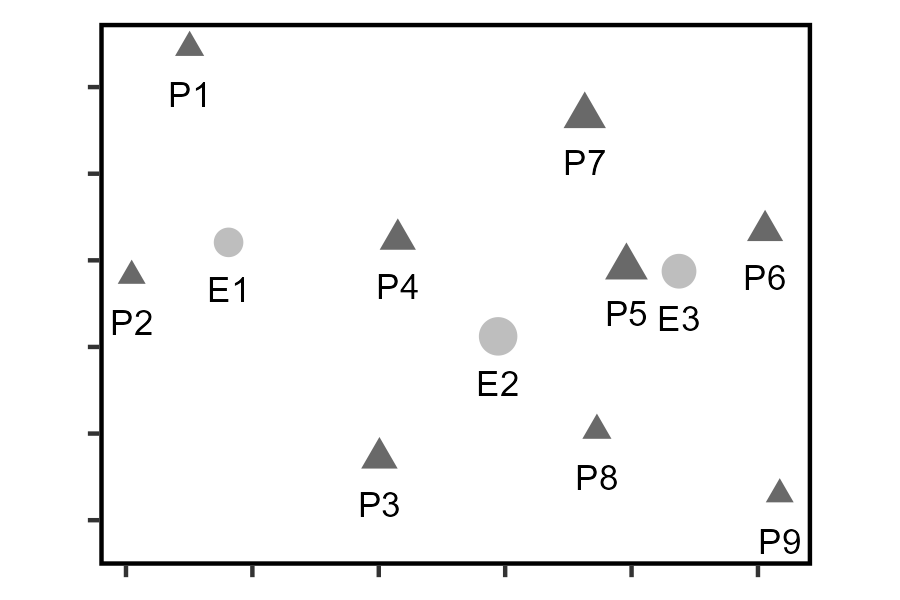
\includegraphics{images/figure-1.png}}\\
\bottomrule
\end{tabular}
\end{table}

\begin{figure}
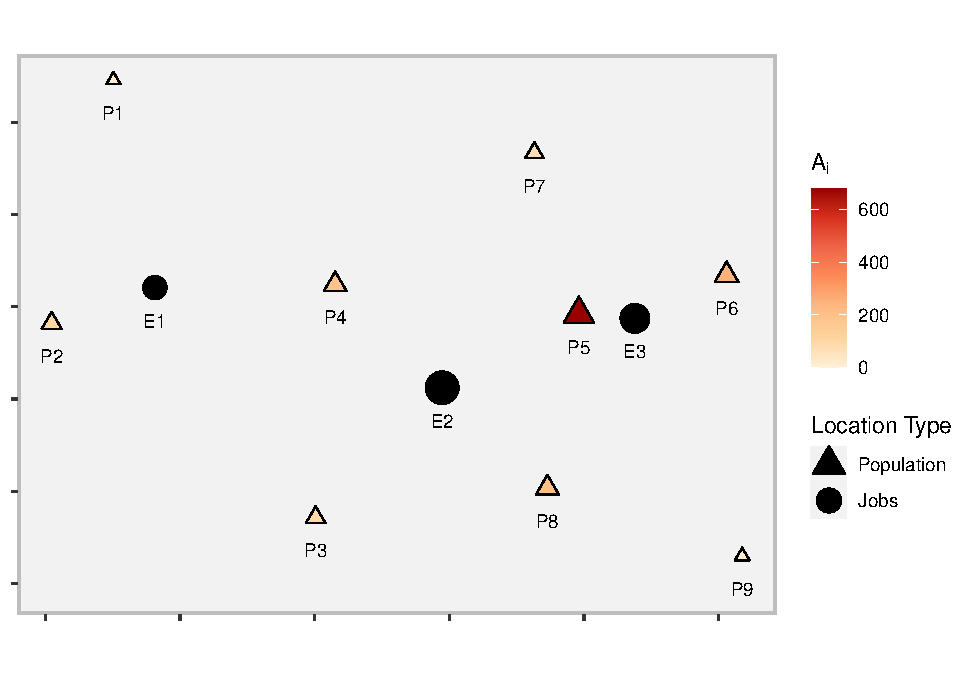
\includegraphics[width=1\linewidth]{Spatial-Availability_files/figure-latex/toy-example-accessibility-plot-1} \caption{\label{fig:toy-example-accessibility}Accessibility to jobs from population centers in the synthetic example}\label{fig:toy-example-accessibility-plot}
\end{figure}

Figure \ref{fig:toy-example-accessibility} shows the locations of the
three employment centers (black circles), where the size of the symbol
is in proportion to the number of jobs at each location. We also see
nine population centers (triangles), where the size of the symbol is
proportional to the accessibility (\(A_i\)) to jobs. The accessibility
values illustrate the following:

\begin{itemize}
\item
  Population centers (triangles) in the middle of the plot are
  relatively close to all three employment centers and thus have the
  highest levels of job accessibility. Population center P5 is
  relatively central and close to all employment centers, and it is the
  closest population to the second largest employment center in the
  region. Unsurprisingly, this population center has the highest
  accessibility 680.64);
\item
  Population centers (triangles) near the left edge of the map (only in
  proximity to the small employment center) have the lowest levels of
  job accessibility. Population center P1 is quite peripheral and the
  closest employment center is also the smallest one. Consequently, it
  has the lowest accessibility with \(A_i=\) 17.12);
\end{itemize}

\hypertarget{the-effect-of-competition-for-opportunities}{%
\subsection{The effect of competition for
opportunities}\label{the-effect-of-competition-for-opportunities}}

Accessibility measures are excellent indicators of the intersection
between urban structure and transportation infrastructure (Kwan, 1998;
Reggiani et al., 2011; Shi et al., 2020). However, beyond enabling
comparisons of relative values they are not highly interpretable on
their own (Miller, 2018). For instance, from Figure
\ref{fig:toy-example-accessibility}, P1 has lower accessibility than P5
but despite the accessibility value for P1 being relatively low it is
still better than \emph{zero}. On the other hand, P5 has high
accessibility, but is its accessibility excellent, good, or only fair?
What does it \emph{mean} for a location to have accessibility to so many
jobs?

To address this interpretability issue, previous research has aimed to
index and normalize values on a per demand-population basis (e.g.,
Barboza et al., 2021; Pereira et al., 2019; Wang et al., 2021). However,
as recent research on accessibility discusses (Allen and Farber, 2019;
Paez et al., 2019), these steps do not address the bias introduced
through the uneven multiple-counting of opportunities and/or population.
This is similar to the congestion effect that floating catchment area
methods aim to address, although these methods do not necessarily solve
the issue completely (see Paez et al., 2019). The underlying issue
arises as a result of the assumption that for conventional accessibility
\(A_i\) all opportunities are \emph{available} to anyone from any origin
\(i=1,\cdots,n\) who can reach them: in other words, they are assumed to
be infinitely divisible and non-competitive. This results in every
opportunity entering the weighted sum once for every origin \(i\) that
can reach it. Put another way, if a densely populated population center
pops up next to P5 this center too will have a high accessibility score
since \(A_i\) does not consider competition of opportunities from
neighbouring population centers. Neglecting to constrain opportunity
counts (i.e., single-constraint) in addition to obscuring the
interpretability of accessibility can also bias results in two ways:

\begin{enumerate}
\def\labelenumi{\arabic{enumi})}
\item
  Demand centers in less dense outer limits of cores may be assigned
  disproportionately \emph{high} accessibility values. These periphery
  areas are traditionally located in proximity to more dense urban
  demand centers and large urban opportunity centers and thus may have
  low travel cost to these large opportunity centers. Accessibility
  \(A_i\) does not consider opportunity-constraints and, as such, these
  periphery demand centers benefit from the high accessibility to
  opportunities without competition considerations from their more dense
  and more centrally located neighbours.
\item
  Remote areas which are still within the region of the analysis and are
  near relative smaller opportunity centers may be assigned
  disproportionately \emph{low} accessibility values, despite facing low
  competition for opportunities. These more remote areas may be
  sufficiently supplied with opportunities proportionate to their demand
  but this relationship is obscured by the artificially high
  accessibility awarded to demand- and opportunity-rich areas in which
  competition disproportionately occurs.
\end{enumerate}

The spatially uneven multiple-counting of opportunities (i.e., the
competition effect) makes accessibility estimates difficult. Recent
accessibility measures which seek to improve interpretability are either
vulnerable to this impact or require heroic assumptions. As previously
mentioned, the floating catchment areas (FCA) method increases
interpretability by purporting to account for competition, however, as
discussed by Paez et al. (2019), FCA methods are vulnerable to a similar
multiple-counting effect. On this same note, the doubly-constrained
gravity model proposed by Allen and Farber (2019) which is based on the
FCA method, accounts for competition, but requires that the magnitude of
demand matches the opportunities or be re-scaled to match. As noted,
this assumption is not always realistic for many opportunity types such
as in the case of job seekers and jobs.

To address the competition effect and to more accurately treat
non-divisible opportunities, we propose a singly-constrained gravity
measure called \textbf{spatial availability}. This measure seeks to
address the following questions from the perspective of an individual at
a specific demand center: \emph{``many opportunities are accessible, but
the same opportunities are also accessible to my (possibly) numerous
neighbors\ldots{} what does high accessibility actually mean to me?''}
and \emph{``few opportunities are accessible to me but I am located in a
remote area with proportionally few neighbors\ldots{} what does low
accessibility mean to me?''}. Beyond the individual, spatial
availability, can also be used as-is to evaluate the \emph{spatial
mismatch} of accessible opportunities and demand-seeking population
within regions and between regions.

\hypertarget{analytical-framework}{%
\section{Analytical framework}\label{analytical-framework}}

Next, we introduce the analytical framework of spatial availability and
highlight the differences between the measures to demonstrate how the
proposed method improves the interpretability of opportunity access.

Formally, spatial availability \(V_{ij}\) is defined by the number of
opportunities \(O\) that are proportionally allocated based on a
population allocation factor \(F^p_{ij}\) and cost of travel allocation
factor \(F^c_{ij}\) for all origins \(i\) to all destinations \(j\) as
detailed in Equation (\ref{eq:spatial-availability}). In line with the
tradition of gravity modeling, the proposed framework distinguishes
between opportunities at a destination and demand for opportunities at
the origin.

\begin{equation}
\label{eq:spatial-availability}
V_{ij} = O_j\frac{F^p_{ij} \cdot F^c_{ij}}{\sum_{i=1}^K F^p_{ij} \cdot F^c_{ij}}
\end{equation}

The terms in Equation \ref{eq:spatial-availability} are as follows:

\begin{itemize}
\tightlist
\item
  \(V_{ij}\) is the spatial availability of opportunities in \(j\) to
  origin \(i\).
\item
  \(i\) is a set of origin locations in the region \(K\).
\item
  \(j\) is a set of destination locations in the region \(K\).
\item
  \(O_j\) is the number of opportunities at location \(j\) in the region
  \(K\).
\item
  \(F^p_{ij}\) is a proportional allocation factor of the population in
  \(i\).
\item
  \(F^c_{ij}\) is a proportional allocation factor of travel cost for
  \(i\); it is a product of a monotonically decreasing (i.e., impedance)
  function associated with the cost of travel between \(i\) and \(j\).
\end{itemize}

Notice that, unlike \(A_i\) in Equation
(\ref{eq:conventional-accessibility}), the population in the region
enters the calculation of \(V_{ij}\). It is important to detail the role
of the two proportional allocations factors in the formulation of
spatial availability. We begin by considering the population allocation
factor \(F^p_{ij}\) followed by the role of the travel cost allocation
factor \(F^c_{ij}\); finally we show how both allocation factors combine
in the final general form of spatial availability \(V_{ij}\). The
calculation of spatial availability is introduced with a step-by-step
example for two population centers (\(P_1\) and \(P_2\)) in the role of
demand (i.e., the number of individuals in the labor market who `demand'
employment) and one employment center (\(O_1\)) in the role of
opportunities.

\hypertarget{population-and-travel-cost-allocation-factors}{%
\subsection{Population and travel cost allocation
factors}\label{population-and-travel-cost-allocation-factors}}

We begin with allocation based on demand by population; consider an
employment center \(j\) with \(O_j^r\) jobs of type \(r\). In the
general case where there are \(K\) population centers in the region, we
define the following factor:

\begin{equation}
\label{eq:pop-alloc-factor}
F^p_{ij} = \frac{P_{i\in r}^\alpha}{\sum_{i=1}^K P_{i\in r}^\alpha}
\end{equation}

The population allocation factor \(F^p_{ij}\) corresponds to the
proportion of the population in origin \(i\) relative to the population
in the region. On the right hand side of the equation, the numerator
\(P_{i\in r}\) is the population at origin \(i\) that is eligible for
and `demands' jobs of type \(r\) (e.g., those with a certain level of
training or in a designated age group). The summation in the denominator
is over \(i=1,\cdots,K\), the population at origins \(i\) in the region.
To modulate the effect of demand by population in this factor we include
an empirical parameter \(\alpha\) (i.e., \(\alpha <1\) places greater
weight on smaller centers relative to larger ones while \(\alpha>1\)
achieves the opposite effect). This population allocation factor
\(F^p_{ij}\) can now be used to proportionally allocate a share of the
jobs at \(j\) to origins.

More broadly, since the factor \(F^p_{ij}\) is a proportion, when it is
summed over \(i=1,\cdots,K\) it always equals to 1 (i.e.,
\(\sum_i^{K} F^p_{ij} = 1\)). This is notable since the share of jobs
(the spatial availability based on population \(V^p_{ij}\)) at each
destination \(j\) allocated to (i.e., available to) each origin is equal
to \(V^p_{ij} = O_j \cdot F^p_{ij}\) and since the sum of \(F^p_{ij}\)
is equal to 1 it follows that \(\sum_{i=1}^I V_{ij} = O_j\). In other
words, the number of jobs across the region is preserved. The result is
a proportional allocation of jobs (opportunities) to origins based on
the size of their populations.

To illustrate the population allocation factor, suppose that the
employment center in the example has 300 jobs (\(O_1= 300\)), and that
the two population centers have 240 and 120 people, respectively,
(\(P_1= 240\) and \(P_2 = 120\)). For simplicity, assume that all the
population in the region is eligible for these jobs, that is, that the
entirety of the population is included in the set \(r\). Also assume
that \(\alpha=1\). The population allocation factors \(F^p_{ij}\) for
the jobs at \(O_1\) for each population center \(P_1\) and \(P_2\) are
as shown in Equation (\ref{eq:pop-alloc-factor-2populations}).

\begin{equation}
\label{eq:pop-alloc-factor-2populations}
\begin{array}{l}\
F^p_{1,1} = \frac{P_1 ^\alpha}{P_1^\alpha + P_2^\alpha} = \frac{240}{240 + 120} = \frac{240}{360}\\
F^p_{2,1} = \frac{P_2^\alpha}{P_1^\alpha + P_2^\alpha}  = \frac{120}{240 + 120} = \frac{120}{360}\\
\end{array}
\end{equation}

These \(F^p_{ij}\) values can be used to find a \emph{partial} spatial
availability in which jobs are allocated proportionally to population;
this partial spatial availability \(V^p_{ij}\) for each population
center is calculated as follows in Equation
(\ref{eq:pop-alloc-factor-SA-2populations}).

\begin{equation}
\label{eq:pop-alloc-factor-SA-2populations}
\begin{array}{l}\
V^p_{1,1} = O_1 \cdot F^p_{1,1} = 300 \cdot \frac{240}{360} = 200 \\
V^p_{2,1} = O_1 \cdot F^p_{2,1} = 300 \cdot \frac{120}{360} = 100 \\
\end{array}
\end{equation}

When using only the proportional allocation factor \(F^p_{ij}\) to
calculate spatial availability (differentiated here by being defined as
\(V^p_{ij}\) instead of \(V_{ij}\)), proportionally more jobs are
allocated to the bigger population center (i.e., 2 times more jobs as it
is 2 times larger in population). We can also see that the sum of
spatial availability for all population centers is equal to the sum of
jobs, i.e., total opportunities are preserved.

Clearly, using only the proportional allocation factor \(F^p_{ij}\) to
calculate spatial availability does not account for how far population
centers \(P_1\) or \(P_2\) are from employment center \(O_1\). It is the
job of the second allocation factor \(F^c_{ij}\) to account for the
friction of distance, as seen in Equation (\ref{eq:tcost-alloc-factor}).

\begin{equation}
\label{eq:tcost-alloc-factor}
F^c_{ij} = \frac{f(c_{ij})}{\sum_{i=1}^K f(c_{ij})}\\
\end{equation}

\noindent where \(c_{ij}\) is the cost (e.g., the distance, travel time,
etc.) to reach employment center \(j\) from \(i\), and \(f(\cdot)\) is
an impedance function that depends on cost (\(c_{ij}\)); in other words,
this allocation factor \(F^c_{ij}\) serves to proportionally allocate
more jobs to closer locations through an impedance function. To continue
with the example, assume that the impedance function is a negative
exponential function with \(\beta=1\). This parameter modulates the
steepness of the impedance effect and is empirically determined in the
case of positive accessibility, or set by the analyst to meet a preset
condition in the case of normative accessibility (Paez et al., 2012).
Also suppose that the distance from population center \(P_1\) to
employment center \(O_1\) is 0.6 km, and the distance from population
center \(P_2\) to employment center \(O_1\) is 0.3 km. The proportional
allocation factor \(F^p_{ij}\) for the jobs at \(O_1\) for both
population centers \(P_1\) and \(P_2\) is defined as follows in Equation
(\ref{eq:tcost-allocation-factor-2populations}).

\begin{equation}
\label{eq:tcost-allocation-factor-2populations}
\begin{array}{l}\
F^c_{1,1} = \frac{\exp(-\beta \cdot D_{1,1})}{\exp(-\beta \cdot D_{1,1}) + \exp(-\beta \cdot D_{2,1})} = \frac{\exp(-0.6)}{\exp(-0.6) + \exp(-0.3)} = 0.426\\
F^c_{2,1} = \frac{\exp(-\beta \cdot D_{2,1})}{\exp(-\beta \cdot D_{1,1}) + \exp(-\beta \cdot D_{2,1})}  = \frac{\exp(-0.3)}{\exp(-0.6) + \exp(-0.3)} = 0.574\\
\end{array}
\end{equation}

We can see that the proportional allocation factor for \(P_2\) is larger
than \(P_1\) since the cost (i.e., distance) to \(O_1\) is lower. Using
the travel cost proportional allocation factors \(F^c_{ij}\) as defined
in Equation (\ref{eq:tcost-allocation-factor-2populations}), we can
calculate the spatial availability of jobs for each population center
based only on \(F^c_{ij}\) and the jobs available at \(O_1\), as shown
in Equation (\ref{eq:tcost-allocation-factor-SA-2populations})

\begin{equation}
\label{eq:tcost-allocation-factor-SA-2populations}
\begin{array}{l}\
V^c_{1,1} = O_1 \cdot F^c_{1,1} = 300 \times 0.426 = 127.8\\
V^c_{2,1} = O_1 \cdot F^c_{2,1} = 300 \times  0.574 = 172.2\\
\end{array}
\end{equation}

As seen above, spatial availability defined by \(F^c_{ij}\) only (i.e.,
\(V^c_{ij}\)) allocates a larger share of jobs to \(P_2\) since the
population center is closer to \(O_1\). However, as previously
discussed, \(P_2\) has a smaller population than \(P_1\), so \(P_1\)
receives a larger share of jobs when spatial availability when it is
defined by \(F^p_{ij}\) (i.e., \(V^p_{ij}\)). It is necessary to combine
both population and travel cost factors to better reflect demand; these
two components are in line with how demand is conventionally modelled in
accessibility calculations which are re-scaled on a per
demand-population basis or also consider competition (e.g., Allen and
Farber, 2019; Barboza et al., 2021; Yang et al., 2006). Fortunately,
since both \(F^c_{ij}\) and \(F^p_{ij}\) preserve the total number of
opportunities (jobs) as they independently sum to 1, they can be
combined multiplicatively to calculate the proposed spatial availability
(\(V_{ij}\)) which considers demand to be based on both population and
travel cost.

\hypertarget{putting-spatial-availability-together}{%
\subsection{Putting spatial availability
together}\label{putting-spatial-availability-together}}

We can combine the proportional allocation factors by population
\(F^p_{ij}\) and travel cost \(F^c_{ij}\) and calculate spatial
availability \(V_{ij}\) as introduced in Equation
(\ref{eq:spatial-availability}) and repeated below:

\[
V_{ij} = O_j\frac{F^p_{ij} \cdot F^c_{ij}}{\sum_{i=1}^K F^p_{ij} \cdot F^c_{ij}}
\]

To complete the illustrative example of employment center \(O_1\) and
population centers \(P_1\) and \(P_2\), the resulting spatial
availability \(V_{ij}\) is calculated for both population centers is
calculated in Equation (\ref{eq:SA-2populations}).

\begin{equation}
\label{eq:SA-2populations}
\begin{array}{l}\
V_{1,1} = O_1\cdot \frac{F^p_{1,1} \cdot F^c_{1,1}}{F^p_{1,1} \cdot F^c_{1,1} + F^p_{2,1} \cdot F^c_{2,1}} = 300 \frac{\big(\frac{2}{3} \big) \big(0.426 \big)}{\big(\frac{2}{3} \big) \big(0.426 \big) + \big(\frac{1}{3} \big) \big(0.574 \big)} = 179.4\\
V_{2,1} = O_1\cdot \frac{F^p_{2,1} \cdot F^c_{2,1}}{F^p_{1,1} \cdot F^c_{1,1} + F^p_{ik} \cdot F^c_{ik}} = 300 \frac{\big(\frac{1}{3} \big) \big(0.574 \big)}{\big(\frac{2}{3} \big) \big(0.426 \big) + \big(\frac{1}{3} \big) \big(0.574 \big)}  =  120.6 \\
\end{array}
\end{equation}

In this example, fewer jobs are allocated to population center \(P_1\)
compared to the allocation by population only, to account for the higher
cost of reaching the employment center. On the other hand, distance
alone allocated more jobs to the closest population center (i.e.,
\(P_2\)), but since it is smaller, it also gets a smaller share of the
jobs overall. To reiterate, the sum of jobs at employment center \(O_1\)
that are allocated to population centers \(P_1\) and \(P_2\)
simultaneously based on \emph{population-} and \emph{travel cost}
allocation factors are preserved (i.e., \(V_{1,1} + V_{2,1} = O_1\)).

In the common case that population centers have multiple destination
opportunities \(j\), spatial availability is simply the sum of Equation
(\ref{eq:spatial-availability}) for all opportunities \(J\) (i.e.,
\(V_i = \sum_{j=1}^J V_{ij}\)). The resulting value of \(V_i\)
represents opportunities (e.g., jobs) that can be accessed from origin
\(i\) and that are \emph{not} allocated to any other competing origin:
\(V_i\) is thus the weighted sum of available opportunities. When
comparing \(V_i\) to the singly-constrained gravity model (see Wilson
(1971)), \(V_i\) is the result of constraining \(A_i\) to match one of
the marginals in the origin-destination table, the known total of
opportunities.

Since the sum of opportunities is preserved in the procedures above, it
is possible to calculate an interpretable measure of spatial
availability per capita (lower-case \(v_i\)) as shown in Equation
(\ref{eq:SA-per-capita}).

\begin{equation}
\label{eq:SA-per-capita}
v_i = \frac{V_i}{P_i}
\end{equation}

To complete the illustrative example, the per capita spatial
availability of jobs is calculated in Equation
(\ref{eq:SA-per-capita-2populations}).

\begin{equation}
\label{eq:SA-per-capita-2populations}
\begin{array}{l}\
v_{1,1} = \frac{V_{1,1}}{1_2} =  \frac{179.4}{240} = 0.8\\
v_{2,1} =  \frac{V_{2,1}}{P_2} =  \frac{120.6}{120} = 1.0\\
\end{array}
\end{equation}

We can see that since \(P_2\) is closer to \(O_1\) and has less
competition (as it has a smaller population than \(P_1\)), \(P_2\)
benefits with a higher spatial availability of jobs per job-seeking
population. We can also compare these values to the overall ratio of
jobs-to-population in this region of one job center and two population
centers is \(300/(240 + 120)=\) 0.83.

\hypertarget{empirical-example-spatial-accessibility-and-availability-of-jobs-in-the-ggh}{%
\section{Empirical example: spatial accessibility and availability of
jobs in the
GGH}\label{empirical-example-spatial-accessibility-and-availability-of-jobs-in-the-ggh}}

In this section we use population and employment data from the Golden
Horseshoe Area (GGH). This is the largest metropolitan region in Canada
and includes the cities of Toronto and Hamilton. We present two scales
of analysis. The first example demonstrates how accessibility broadly
overestimates \emph{job access} (relative to spatial availability) and
particularly overestimates job access for areas in the less dense outer
limits of the urban core. The second example demonstrates how
accessibility underestimates job access for areas in the urban
periphery. We first introduce the data used, then calibrate an impedance
function, and finally discuss the results.

\hypertarget{data}{%
\subsection{Data}\label{data}}

Population and employment data are drawn from the 2016 Transportation
Tomorrow Survey (TTS). This survey collects representative urban travel
information from 20 municipalities contained within the GGH area in the
southern part of Ontario, Canada (see Figure
\ref{fig:TTS-16-survey-area}) (Data Management Group, 2018). The data
set includes Traffic Analysis Zones (TAZ) (n=3,764), the number of jobs
(n=3,081,885) and workers (n=3,446,957) at each origin and destination.
The TTS data is based on a representative sample of between 3\% to 5\%
of households in the GGH and is weighted to reflect the population
covering the study area has a whole (Data Management Group, 2018).

To generate the travel cost for these trips, travel times between
origins and destinations are calculated for car travel using the R
package \{r5r\} (Rafael H. M. Pereira et al., 2021) with a street
network retrieved from OpenStreetMap for the GGH area. A the 3 hr travel
time threshold was selected as it captures 99\% of population-employment
pairs (see the travel times summarized in Figure
\ref{fig:TTS-16-survey-area}). This method does not account for traffic
congestion or modal split, which can be estimated through other means
(e.g., Allen and Farber, 2021; Higgins et al., 2021). For simplicity, we
carry on with the assumption that all trips are taken by car in
uncongested travel conditions.

All data and data preparation steps are documented and can be freely
explored in a companion open data product
\href{https://github.com/soukhova/TTS2016R}{\{TTS2016R\}}.

\begin{figure}

{\centering 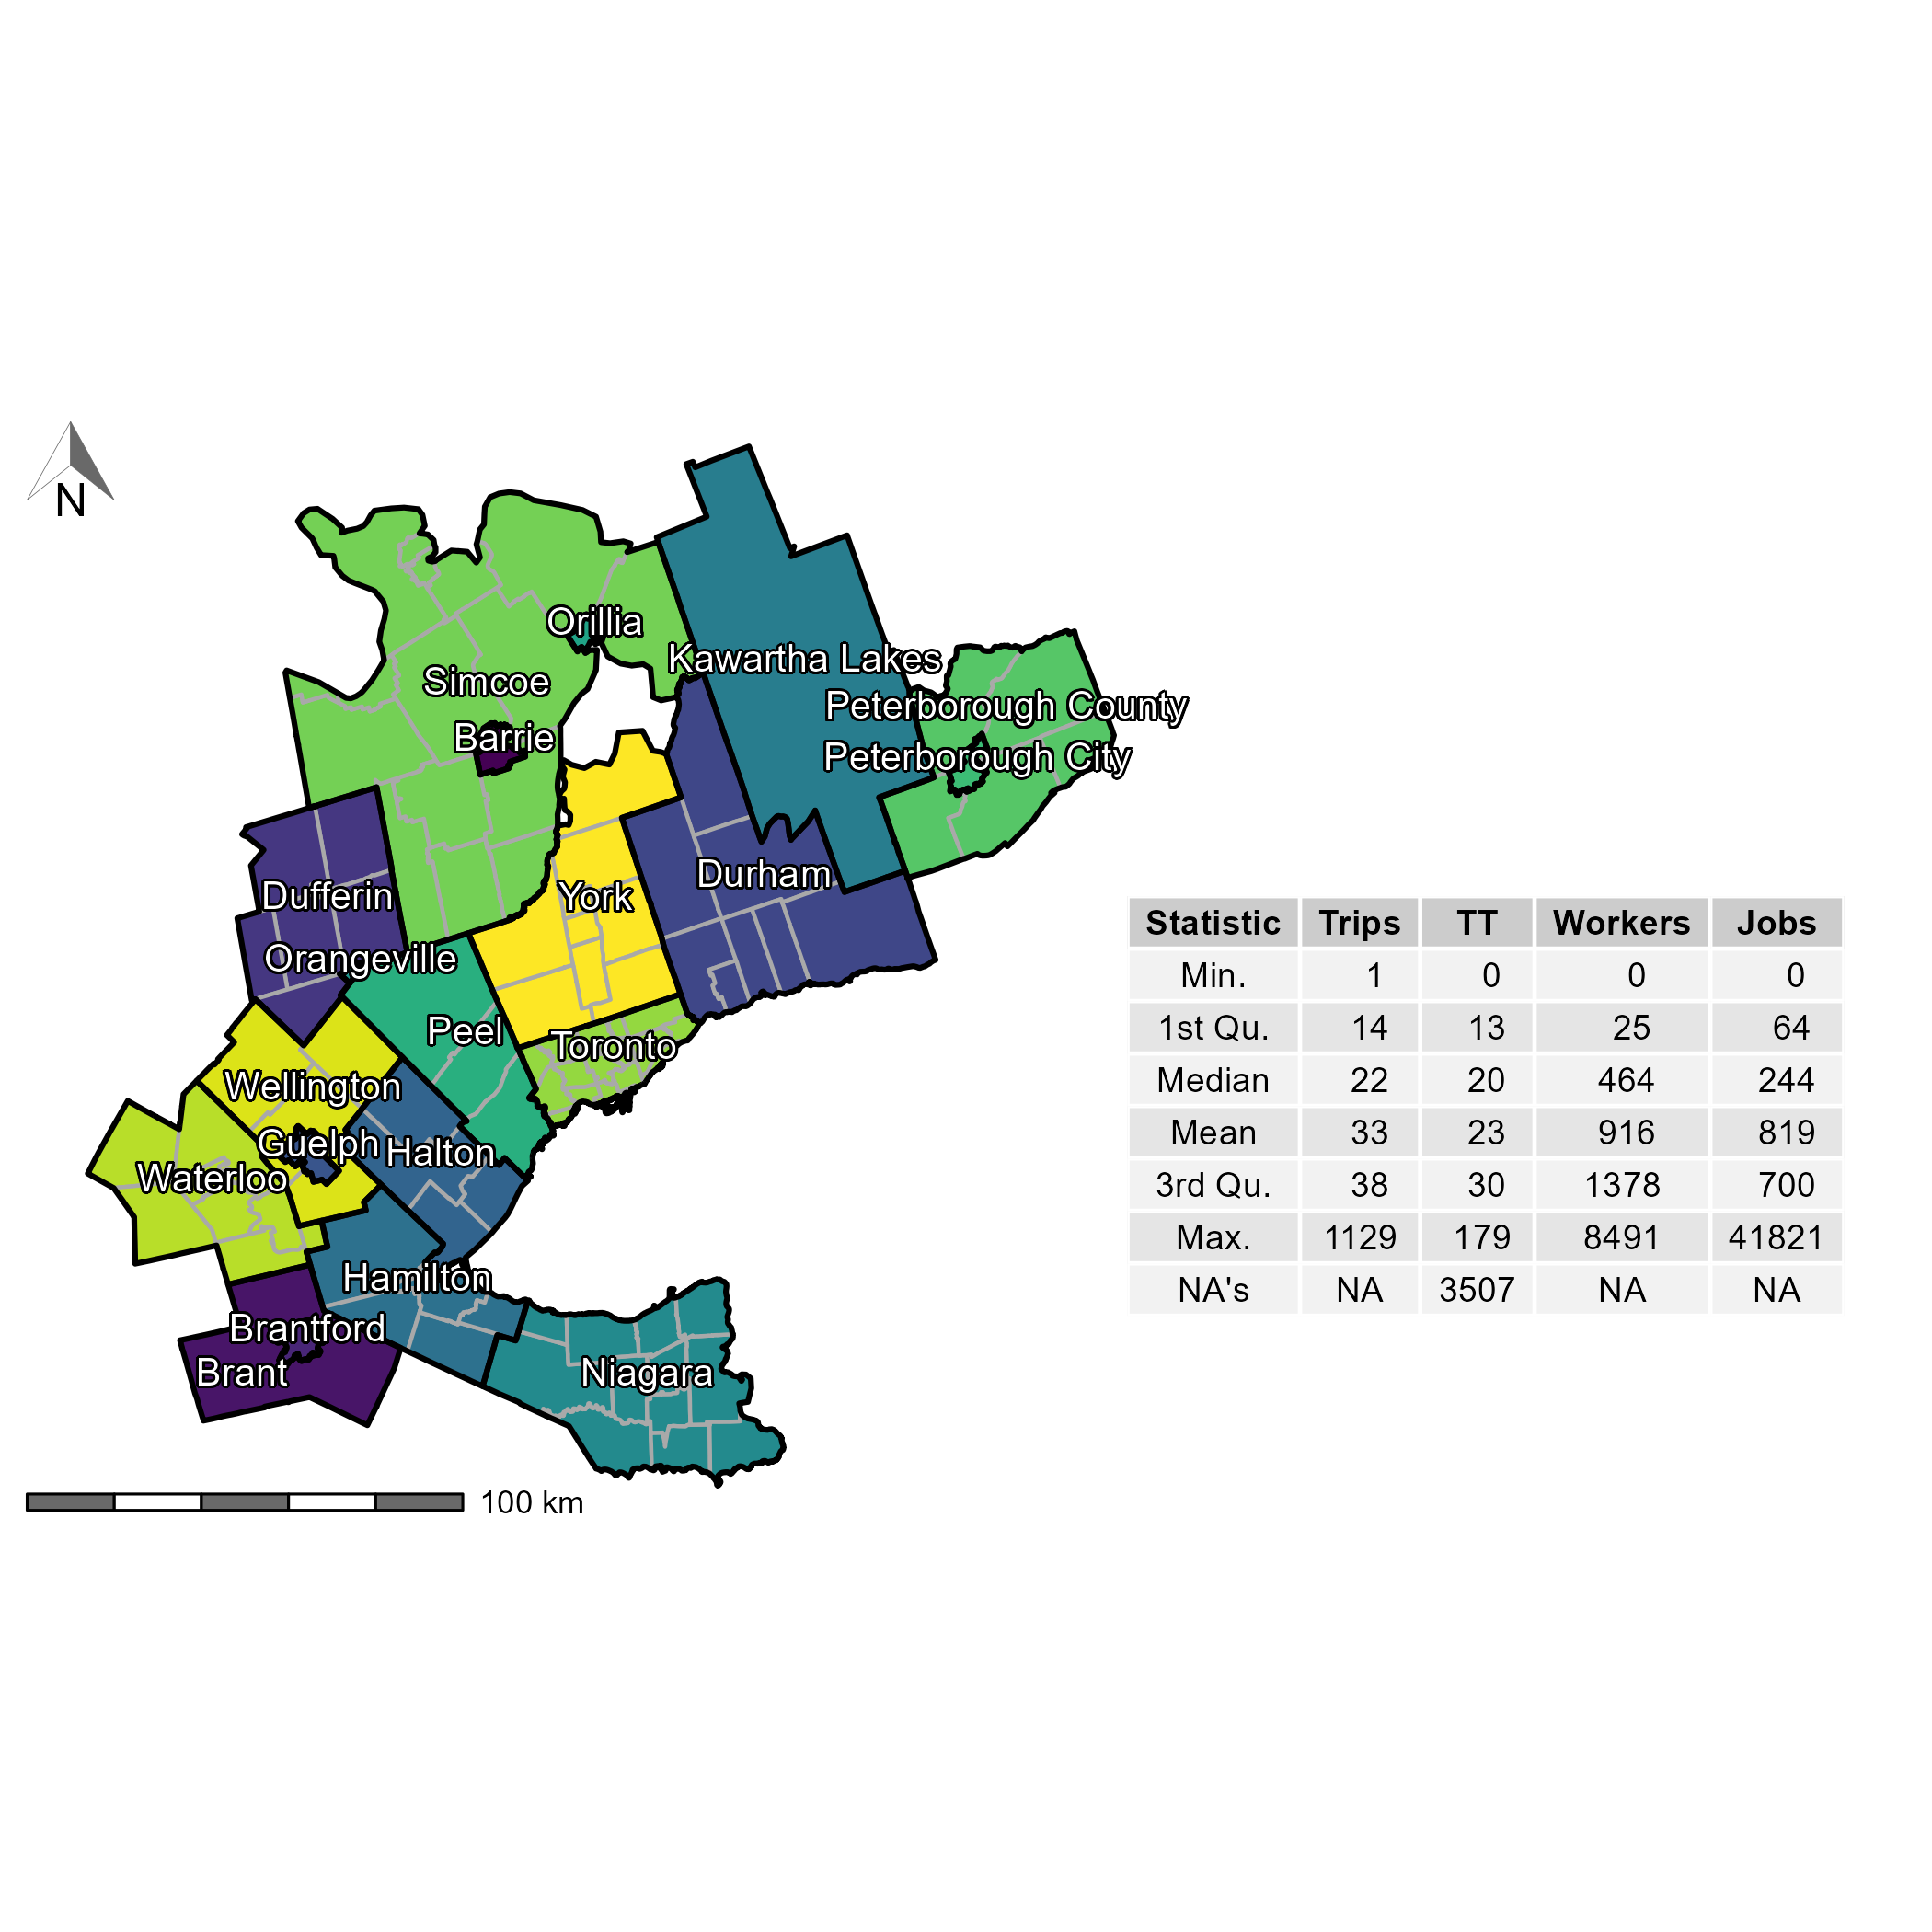
\includegraphics[width=0.8\linewidth]{images/TTS16-survey-area} 

}

\caption{\label{fig:TTS-16-survey-area}TTS 2016 study area within the GGH in Ontario, Canada along with the descriptive statistics of the trips, calculated origin-destination car travel time (TT), workers per TAZ, and jobs per TAZ. Contains 20 regions (black boundaries) and sub-regions (dark gray boundaries).}\label{fig:TTS-16-survey-area}
\end{figure}

\hypertarget{calibration-of-an-impedance-function}{%
\subsection{Calibration of an impedance
function}\label{calibration-of-an-impedance-function}}

In the synthetic example introduced in a preceding section, a negative
exponential function with an arbitrary parameter was used. For the
empirical example, we calibrate an impedance function on the trip length
distribution (TLD) of commute trips. Briefly, a TLD represents the
proportion of trips that are taken at a specific travel cost (e.g.,
travel time); this distribution is commonly used to derive impedance
functions in accessibility research (Batista et al., 2019; Horbachov and
Svichynskyi, 2018).

The empirical and theoretical TLD for this data set are represented in
the top-left panel of Figure \ref{fig:TLD-Gamma-plot}. Maximum
likelihood estimation and the Nelder-Mead method for direct optimization
available within the \texttt{fitdistrplus} package (Delignette-Muller
and Dutang, 2015) were used. Based on goodness-of-fit criteria and
diagnostics seen in Figure \ref{fig:TLD-Gamma-plot}, the gamma
distribution was selected (also see Figure \ref{fig:plot-cullen-frey} in
Appendix A).

\begin{figure}

{\centering 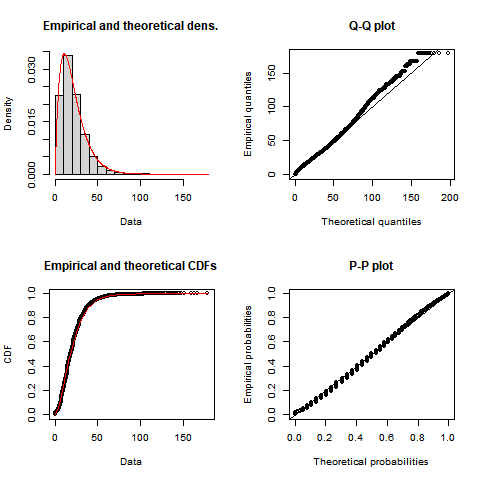
\includegraphics[width=1\linewidth]{images/impedance_function} 

}

\caption{\label{fig:TLD-Gamma-plot}Empirical TTS 2016 home-based car trip length distribution (black points) and calibrated gamma distribution impedance function (red line) with associated Q-Q and P-P plots}\label{fig:TLD-Gamma-plot}
\end{figure}

The gamma distribution takes the following general form where the
estimated `shape' is \(\alpha=\) 2.019, the estimated `rate' is
\(\beta =\) 0.094, and \(\Gamma(\alpha)\) is defined in Equation
(\ref{gamma-dist}).

\begin{equation}
\label{gamma-dist}
\begin{array}{l}\ 
f(x, \alpha, \beta) = \frac {x^{\alpha-1}e^{-\frac{x}{\beta}}}{ \beta^{\alpha}\Gamma(\alpha)} \quad \text{for } 0 \leq x \leq \infty\\

\Gamma(\alpha) =  \int_{0}^{\infty} x^{\alpha-1}e^{-x} \,dx\\
\end{array}
\end{equation}

\hypertarget{measuring-access-to-jobs-in-the-ggh}{%
\subsection{Measuring access to jobs in the
GGH}\label{measuring-access-to-jobs-in-the-ggh}}

Toronto is the largest city in the GGH and represents a significant
subset of workers and jobs in the GGH; 51\% of workers in the GGH travel
to jobs in Toronto and 73\% of jobs are located within Toronto. As will
be discussed, when accessibility and spatial availability values are
compared, this significant subset of jobs in Toronto illustrates both
issues associated with the competition effect. Specifically, since
accessibility does not include the single-opportunity constraint like
spatial availability does, it \emph{overestimates} the jobs available
for most TAZs in proximity to Toronto (i.e., GTA) and
\emph{underestimates} the jobs available for TAZs in the periphery of
the GGH.

Figure \ref{fig:plot-access-SA-GGH-TTS} presents the accessibility and
spatial availability for the full TTS data set. Conventionally, higher
accessibility is interpreted as the ability to reach more opportunities.
Within the accessibility plot, job access values follow a radial trend
where a few TAZ with a high values are strictly located within the
boundaries of Toronto and values radially decrease further from the
boundaries of Toronto. This general trend is echoed in qualitative
studies which find the further from Toronto the longer the employment
commute (Axisa et al., 2012) and the closer to core of Toronto the more
opportunities are accessible (for some to certain types of jobs, see
Páez et al., 2013).

Next, spatial availability measure and is presented alongside the
accessibility plot in Figure \ref{fig:plot-access-SA-GGH-TTS}. Similar
to the accessibility plot, the higher the value, the more access that
TAZ has to jobs in the GGH. Since spatial availability constrains the
total to match the number of opportunities, high values of spatial
availability can be seen as higher access to \emph{available} jobs
(i.e., competitive job access) and we can observe which TAZs have
spatial availability values which are above or below the regional
average of 642. It is worth noting that the spatial availability and
accessibility plots do not follow the same spatial distribution. Within
the spatial availability plot, job access appears more evenly assigned
throughout the GGH. Particularly, job access values, as measured by
spatial availability, are higher around the north east and south west
periphery TAZs and more moderate in and around Toronto than compared to
accessibility.

Note that in Figure \ref{fig:plot-access-SA-GGH-TTS} it can be observed
that a few TAZ are greyed out; this corresponds to a null accessibility
and spatial availability. Overall, 22\% of TAZ are greyed out as a
result of containing zero home-to-work GGH trips and as such are
allocated a null accessibility and spatial availability. The majority of
these no-trip TAZ because they contain no worker population,
specifically, 95\% have zero workers while only 18\% of these TAZ have
zero jobs (17\% have both zero workers and jobs).

\begin{figure}
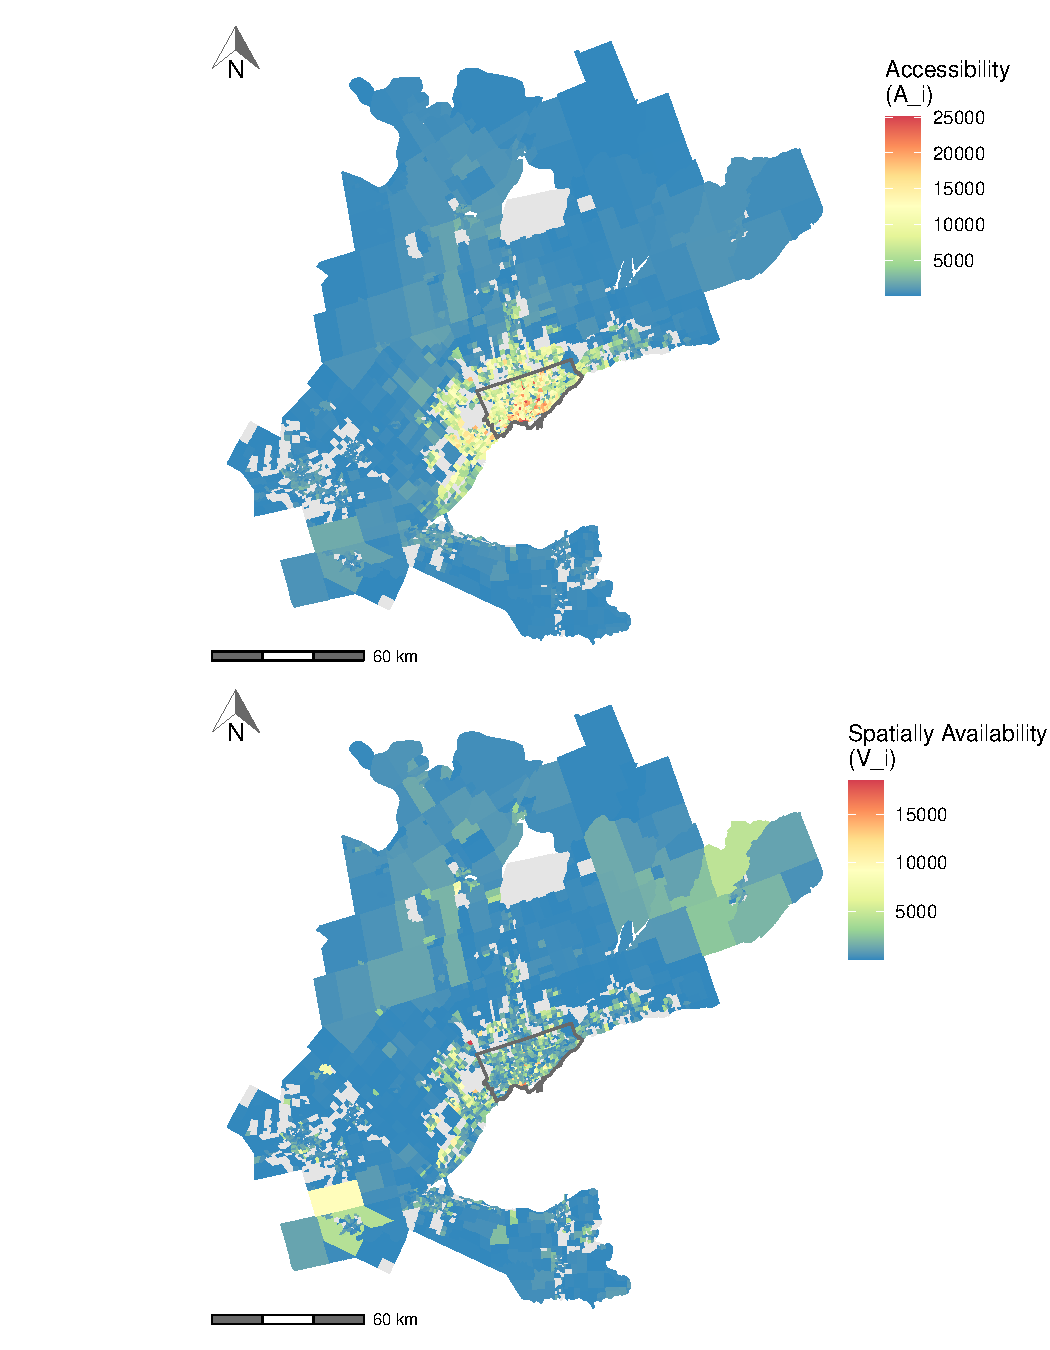
\includegraphics[width=1\linewidth]{Spatial-Availability_files/figure-latex/plot-access-SA-GGH-TTS-1} \caption{\label{fig:plot-access-SA-GGH-TTS}Calculated accessibility (top) and spatial availability (bottom) of employment from origins in the GGH to destinations in the GGH. Greyed out TAZs represent null accessibility and spatial availability values .}\label{fig:plot-access-SA-GGH-TTS}
\end{figure}

\newpage

To enhance the interpretability of spatial availability, the measure can
be normalized to provide more meaningful insight into how many jobs are
\emph{available} on average for each TAZ. This normalization, shown in
Figure \ref{fig:plot-avail-GGH-TTS-per-worker}, demonstrates which TAZ
have above (reds) and below (blue) the average ( available jobs per
worker in the GGH. Similar to the spatial availability plot of the GGH
jobs in Figure \ref{fig:plot-access-SA-GGH-TTS}, we can see that many
average or above average jobs per worker TAZ (whites and reds) are
present in southern Peel and Halton (south-west of Toronto), Waterloo
and Brantford (even more south-west of Toronto), and Hamilton and
Niagara (south of Toronto), however, the distribution is uneven and many
TAZ within these areas do have below average values (blues).

Interestingly, when considering \emph{competitive} job access, many
areas outside of Toronto have similar jobs per worker values as TAZ in
Toronto. This is contrary to the notion that since Toronto has high job
access it has a significant density of employment opportunities in the
GGH. Not all jobs in Toronto are \emph{available} since Toronto has a
high density of \emph{competition} in addition to density of jobs
opportunities. For instance, urban centers outside of Toronto such as
those found in Brantford, Guelph, southern Peel, Halton, and Niagara
have TAZ which are far above the the TTS average jobs per worker and
higher than TAZ within Toronto. High job access is not seen in the
accessibility plot which suggests that these less densely populated
urban centers may have sufficient employment opportunities for their
populations; This finding is obscured when only considering the
accessibility measure for job access as will be later discussed.

It is also worth noting that there is almost two times more jobs per
worker in the GGH jobs spatial availability results than the GGH Toronto
spatial availability results. This suggests that all GGH people who work
in the city of Toronto, on average, face more competition for jobs than
all GGH people who work anywhere in the GGH .

\begin{figure}
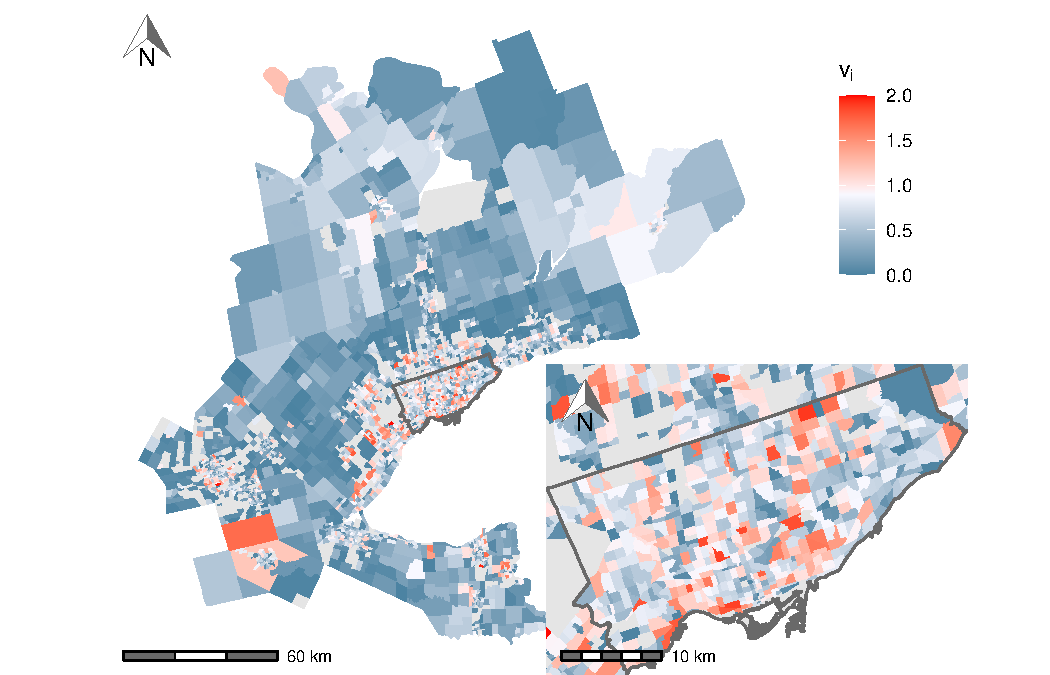
\includegraphics[width=1\linewidth]{Spatial-Availability_files/figure-latex/plot-avail-GGH-TTS-per-worker-1} \caption{\label{fig:plot-avail-GGH-TTS-per-worker}Spatial availability per worker, from origins to job opportunities in the GGH.}\label{fig:plot-avail-GGH-TTS-per-worker}
\end{figure}

\newpage

\hypertarget{discussion}{%
\section{Discussion}\label{discussion}}

In the preceding section we used both spatial accessibility and
availability measures to explore the landscape of employment
opportunities in the GGH. To build on these findings, we return to the
two issues associated with spatial accessibility. As noted earlier,
accessibility has the tendency to overestimate the number of
opportunities in areas with high competition (issue 1) and underestimate
the number of opportunities in areas with low competition (issue 2).

To compare both accessibility and spatial availability, we calculate
their relative magnitudes by re-scaling both measures from 0 to 100
where each value of the measure is divided by the maximum value as
described in Equation \ref{eq:index-measures} by \(A^I_{ij}\) and
\(V^I_{ij}\). Re-scaling is repeated for both measures and the
proportional difference between the measures is calculated as described
in Equation \ref{eq:dif-index-measures}. This difference represents how
many times over- or under- estimates the number of jobs for a TAZ when
measured by the re-scaled accessibility relative to the re-scaled
spatial availability (e.g., accessibility is X times \emph{larger} than
spatial availability thus job access is \emph{overestimated} when using
the accessibility measure compared to the spatial availability measure).

\begin{equation}
\label{eq:index-measures}
\begin{array}{l}\
A^I_{ij} = \frac{A_{ij}}{\max(A_{ij})}\cdot100\\
V^I_{ij} = \frac{V_{ij}}{\max(V_{ij})}\cdot100\\
\end{array}
\end{equation}

\begin{equation}
\label{eq:dif-index-measures}
\Delta_{ij} = \frac{A^I_{ij}}{V^I_{ij}}
\end{equation}

\hypertarget{over--and-under-estimation-of-opportunities-in-space-by-accessibility-measures}{%
\subsection{Over- and under-estimation of opportunities in space by
accessibility
measures}\label{over--and-under-estimation-of-opportunities-in-space-by-accessibility-measures}}

Here we explore the difference between the two measures for the full
data set, namely, all jobs within the GGH and all workers within the
GGH. While the majority of TAZ have difference values which correspond
to accessibility being overestimated relative to spatial availability,
83\% of TAZ are underestimated.

The overestimated TAZ have a median difference of 4.43 which indicates
that the median accessibility value over-estimates the median spatial
availability by 4.43 times. Differences when overestimating the number
of opportunities ranges between 1 to 1889 with an upper quartile value
(75\%) of 10.54. It should be noted that these TAZ with an upper 95\% of
difference values (69 to 1889) are a result of high competition and/or
high multiple-counting of opportunities; They contain exceptionally low
spatial availability values and relatively high accessibility values.

Conversely, a few TAZ are underestimated and are plotted in Figure
\ref{fig:plot-difference-GGH} alongside the overestimated TAZ for
comparison. Of the underestimated TAZ, the median spatial availability
value is 0.605 indicating that the median accessibility is 0.605 the
spatial availability value. The difference values ranges between 0.006
to 0.995.

\begin{figure}
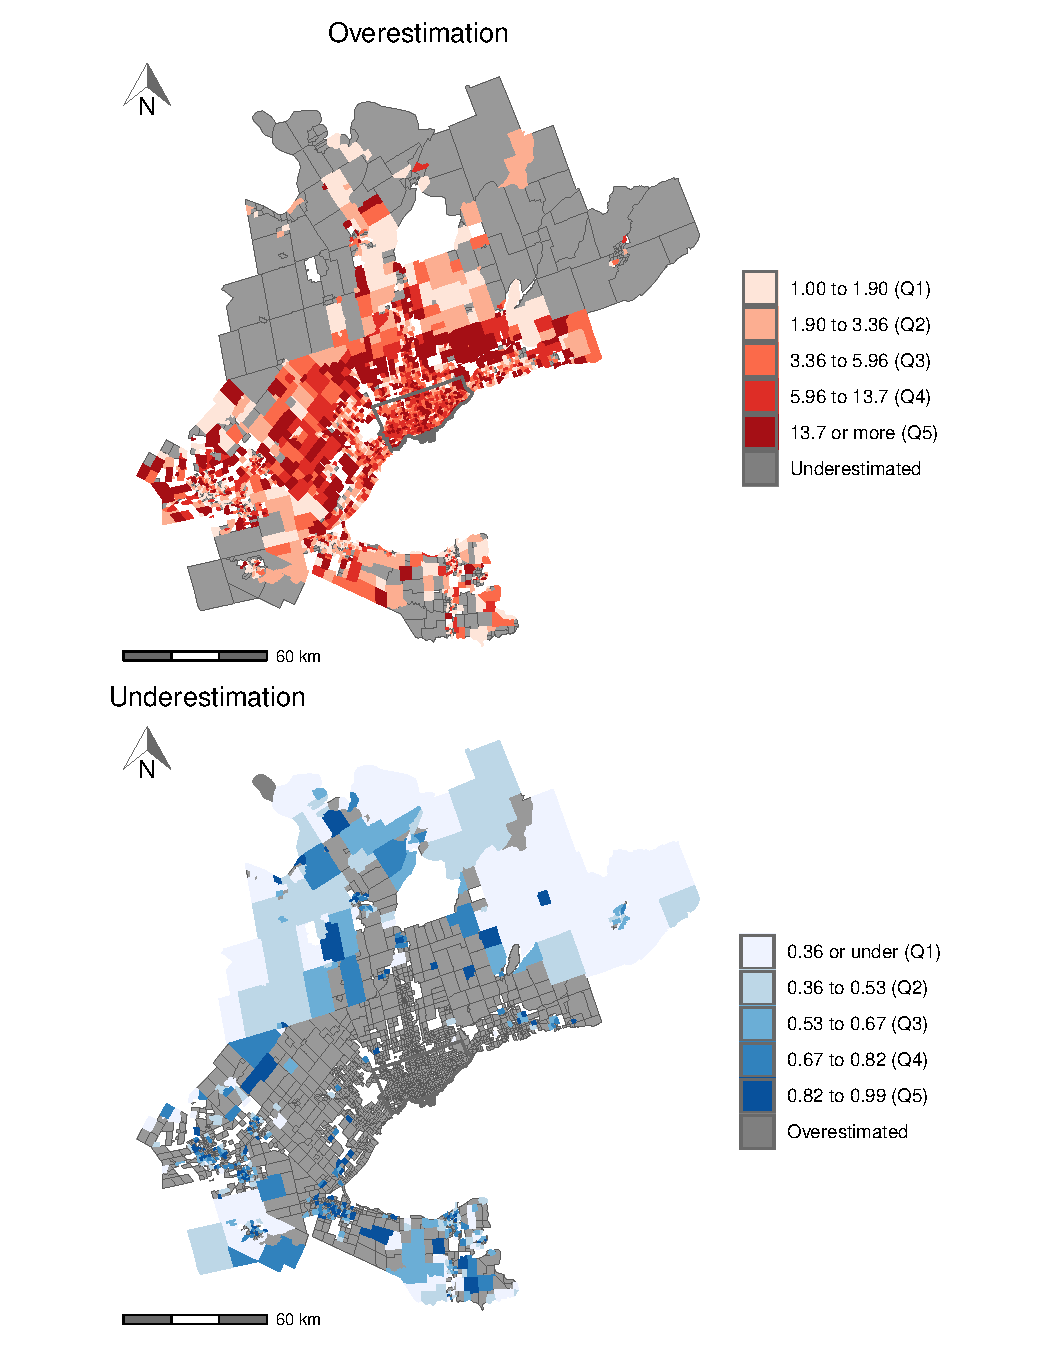
\includegraphics[width=1\linewidth]{Spatial-Availability_files/figure-latex/plot-difference-GGH-1} \caption{\label{fig:plot-difference-GGH}Overestimated (top) and underestimated (bottom) differences between the re-scaled accessibility and spatial availability job access measures in the context of employment from all origins and destinations in the GGH. Values are expressed in five quantile ranges. Greyed TAZs have values which are underestimated in the top plot and are overestimated in the bottom plot. TAZs with no trips and thus no spatial availability or accessibility values are not drawn.}\label{fig:plot-difference-GGH}
\end{figure}

As observed from the top plot in Figure \ref{fig:plot-difference-GGH},
the TAZ with overestimated job access are coloured in varying shades of
red. TAZ with the highest degree of overestimation (darkest reds) are
concentrated within Toronto and the periphery of the GTA. Differences
between the number of workers and travel time partially explain the
overestimation, with TAZs that have a lower number of workers and higher
travel time having a larger overestimation. Specifically, the
correlations between workers and overestimation, and travel time and
overestimation is -0.17 and 0.13 respectively.

Nonetheless, the TAZ-specific density of workers and travel time does
not fully explain the variation in overestimation; the number of
opportunities and the value of these variables in neighbouring TAZ also
factor into the calculation for both measures. From the perspective of
accessibility, since opportunity-constraints are not considered, the
\emph{overestimated} TAZ (relative to spatial availability) are awarded
higher values since they are more centrally located to opportunities
(i.e., low travel cost) and are not discounted from being in proximity
to highly competitive TAZ (i.e., high density of workers). On the other
hand, spatial availability considers this competition by proportionally
allocating jobs to TAZ relative to their travel cost and worker
population. In other words, TAZ appears \emph{overestimated} when the
impact of travel cost alone outpaces the impact of both travel cost and
workers thus the proportional allocation of opportunity results in a
significantly smaller job access than the resulting value for
accessibility. This may explain why TAZ which are exceptionally
overestimated (dark reds) are on the periphery of more densely populated
urban cities. These TAZ are located far enough away from workers in
densely populated TAZ but still relatively close enough to jobs in
Toronto. As such, their high accessibility value is a result of counting
many more opportunities than the single-constrained spatial availability
proportionally allocates. In general, the results suggest that
overestimation of the number of opportunities in accessibility results
from multiple-counting in situations where there is high competition.

Turning to the bottom plot in Figure \ref{fig:plot-difference-GGH}, TAZ
with underestimated job access (i.e., re-scaled accessibility values are
smaller than re-scaled spatial availability values) are located on the
periphery of the GGH area. The majority of these underestimated TAZ are
not within the center of the GGH where the GTA is located but are in
proximity to other, smaller, employment areas within smaller
municipalities. Higher spatial availability results from low job
competition, whereas low accessibility scores simply reflect the lower
density of opportunities. Accessibility's multiple-counting effectively
deflates the job access in these peripheral TAZ since their
accessibility values are significantly lower compared to their
multiple-counted GTA TAZ neighbours. The impact of this
multiple-counting is starkly apparent when compared to the re-scaled
spatial availability measure since spatial availability allocates jobs
proportionally based on workers and travel cost, TAZ do not
multiple-counting of jobs and TAZ which are not in the position to
multiple-count are not deflated as a consequence. This is further
butressed when we examine the spatial availability of jobs per worker in
Figure \ref{fig:plot-avail-GGH-TTS-per-worker}, where we can see that
commercial areas throughout the GGH area have similar job access values
as within some commercial areas in the GTA; this is not the case for the
accessibility measure (see trends in Figure
\ref{fig:plot-access-SA-GGH-TTS}).

\newpage

\begin{figure}
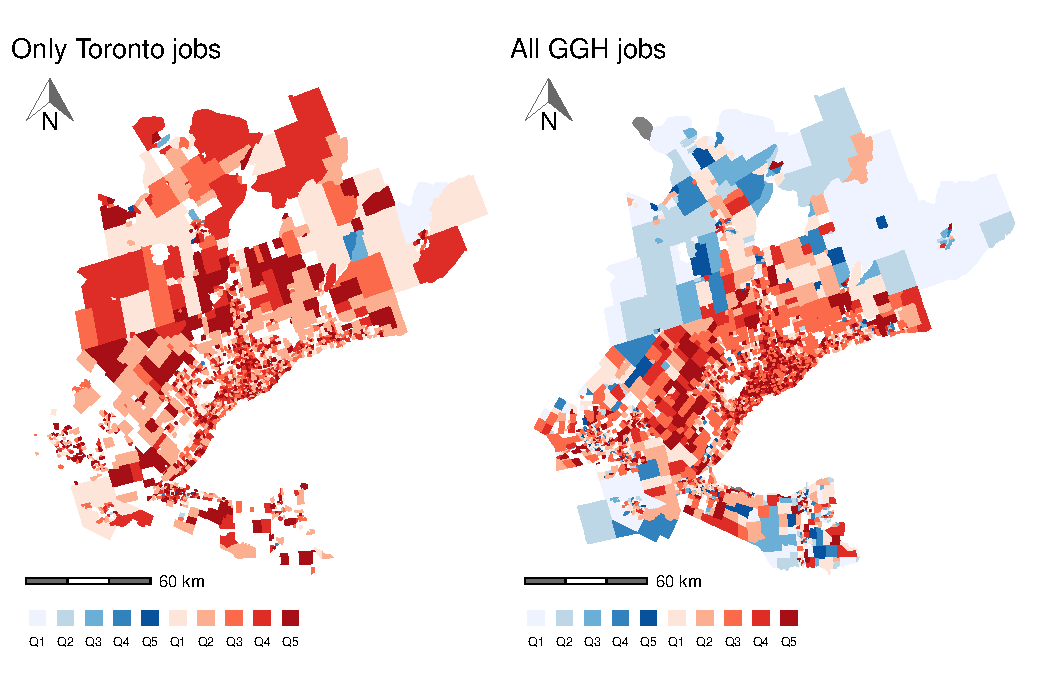
\includegraphics[width=1\linewidth]{Spatial-Availability_files/figure-latex/plot-diff-Toronto-vs-GGH-1} \caption{\label{fig:plot-diff-Toronto-vs-GGH}Overestimated and underestimated difference quantiles between the re-scaled accessibility and spatial availability for Toronto only jobs (left) and all GGH jobs (right). Red represent overestimated differences (i.e., accessibility larger than spatial availability) and blue represents underestimated diffeences (i.e., spatial availability larger than accessibility). TAZs with no trips and thus no spatial availability or accessibility values are not drawn.}\label{fig:plot-diff-Toronto-vs-GGH}
\end{figure}

\hypertarget{differences-in-accessible-and-available-employment-opportunities}{%
\subsection{Differences in accessible and available employment
opportunities}\label{differences-in-accessible-and-available-employment-opportunities}}

Next, we present two additional difference plots in Figure
\ref{fig:plot-diff-Toronto-vs-GGH} as a point of comparison; included is
a consolidated plot of those included in Figure
\ref{fig:plot-diff-Toronto-vs-GGH} and another plot calculated only
using the subset of jobs in Toronto (i.e., all workers in the GGH who
travel to work in a Toronto-located job). This subset of jobs is a
substantial share of employment in the region but are concentrated in
the City of Toronto, which is spatially a small portion of the whole
GGH. Specifically, 51\% of workers in the GGH travel to jobs in Toronto
and 73\% of jobs are located within Toronto. It can be observed, that
when subseting the analysis to \emph{only} include Toronto jobs, almost
all TAZ are overestimated (i.e., accessibility is larger than spatial
availability). Notably, we can see virtually all \emph{underestimation}
disappears (blues) and the TAZs in the GHG periphery are now all
overestimated (reds).

When inspecting the results for the subset of jobs in Toronto and
comparing it to the results of the GGH periphery TAZ within the full GGH
analysis, the effect of the single-constraint of the spatial
availability measure is evident. Looking at the GGH peripheral TAZ in
the left plot (Figure \ref{fig:plot-difference-GGH}), these TAZ have
relatively low spatial availability as they experience moderately high
job competition since they have relatively high travel times to jobs in
Toronto and have a moderately low worker population. Similarly, these
peripheral TAZ also have relatively low accessibility (compared to the
region) as a result of the multiple-counting which occurs within and
around the high density of jobs in Toronto. However, when spatial
availability and accessibility are compared, accessibility is still
\emph{higher} than spatial availability thus the difference appears
\emph{overestimated} (red).

Interestingly, the difference in the two measures flips when the workers
who work in areas outside of Toronto are re-introduced to these
peripheral TAZ as represented in right plot (Figure
\ref{fig:plot-difference-GGH}). Since more workers (more competition)
and more jobs with lower travel costs (less competition) are introduced,
it can be inferred that these peripheral TAZ experience moderately
higher job access as measured with spatial availability. Conversely, for
the accessibility measure, the introduction of additional workers does
not meter the accessibility gained by the introduction of additional
jobs and as such, the re-scaled accessibility values are \emph{higher}
than the spatial availability resulting in underestimated TAZ.

As such, we see that when including all the jobs in the region back into
the analysis - these periphery TAZ are much less \emph{job deprived}
when measured using spatial availabily than when measuring using
accessibility. Overall, within the full set of jobs in the GGH, it is
wasy to see the first and second issues associated with the lack of
competition in accessibility analysis.

\hypertarget{other-use-cases-of-spatial-availability}{%
\section{Other use cases of spatial
availability}\label{other-use-cases-of-spatial-availability}}

In addition to measuring access to jobs for workers, spatial
availability can be used to measure many other opportunity types and
scenarios. In this section we briefly discuss two additional ways in
which spatial availability can be applied in practice. Since spatial
availability singly-constraints opportunities which are allocated to the
demand seeking population, opportunities or demand seeking populations
can be subset while the resulting access measure does not lose any
interpretability. As such, we firstly present an example with
specialized population subsets and specialized employment centers. We
then present an example where the focus is changed to employers seeking
worker.

To illustrate these two additional examples, we return to the synthetic
example initially introduced in Background section.

\hypertarget{specialized-employment-opportunities}{%
\subsection{Specialized employment
opportunities}\label{specialized-employment-opportunities}}

Suppose that population centers P1 through P8 are not all eligible for
employment at the three employment centers E1, E2, and E3. This can be
due to education attainment or more simply a geographic barrier (i.e.,
river without a bridge) making it impossible for certain populations to
be employed at certain employment centers. In this example, we consider
that only population center P1 and P2 are eligible for employment at
employment center E1. Next assume that jobs in employment center E2 can
be taken by individuals in population centers P3, P4, P5, P7, and P8.
Lastly, jobs in employment center E3 require qualifications available
only among individuals in population centers P5, P6, P8, and P9. In
essence, eligibility criteria creates catchments as seen in Figure
\ref{fig:toy-example-availability-with-catchments}.

\begin{figure}
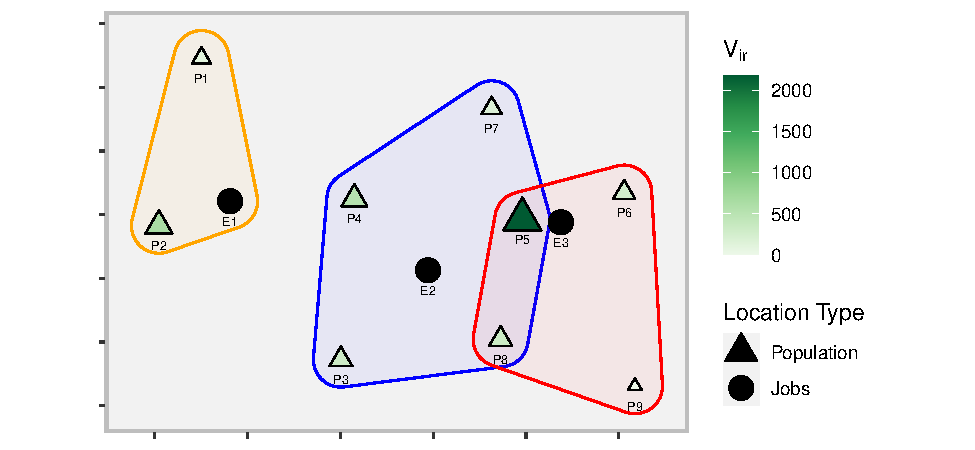
\includegraphics[width=1\linewidth]{Spatial-Availability_files/figure-latex/toy-example-availability-with-catchments-1} \caption{\label{fig:toy-example-availability-with-catchments}Spatial availability of jobs from population centers assuming catchment restrictions (r) for the simple synthetic example}\label{fig:toy-example-availability-with-catchments}
\end{figure}

\begin{figure}
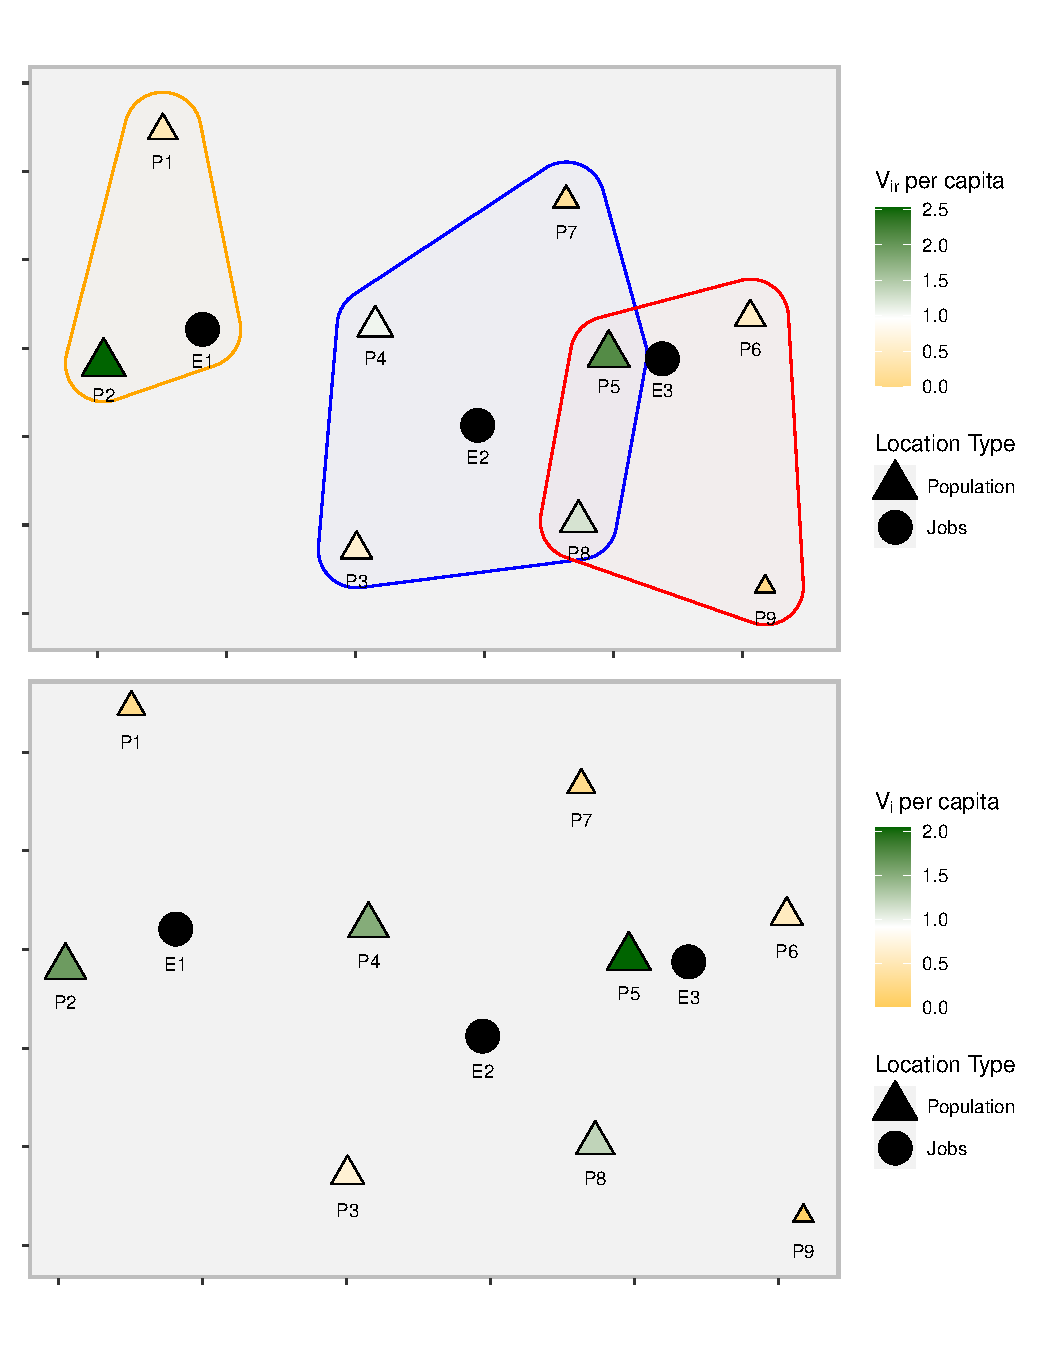
\includegraphics[width=1\linewidth]{Spatial-Availability_files/figure-latex/toy-example-availability-jobs-per-capita-1} \caption{\label{fig:toy-example-availability-jobs-per-capita} Spatial availability of jobs per capita for each population centers with catchment restrictions (r) (top) and without catchment restrictions (bottom) for the synthetic example}\label{fig:toy-example-availability-jobs-per-capita}
\end{figure}

For higher interpretability, we can inspect Figure
\ref{fig:toy-example-availability-jobs-per-capita} which presents plots
of spatial availability per capita with and without catchments.

In the bottom plot of Figure
\ref{fig:toy-example-availability-jobs-per-capita}, we see that
population center P5 has the highest level of spatial availability, due
to being a large population center that is relatively close to jobs. We
also see population centers which are further from employment centers
have low spatial availability (P1, P3, P6, P7, P9) and population
centers which are more central have, evidently, higher job access. We
can also discern that the regional spatial availability per capita is
0.908. In contrast, when catchments are introduced, as shown in the top
plot of Figure \ref{fig:toy-example-availability-jobs-per-capita}, we
see that the number of opportunities available for population centers in
the blue catchment decreases as job competition increases. However, we
also observe that access marginally increases for the population centers
in the yellow catchment and the regional spatial availability per capita
increases slightly to 0.964.

\hypertarget{spatial-availability-of-labor-pool}{%
\subsection{Spatial availability of labor
pool}\label{spatial-availability-of-labor-pool}}

In this use case, we remove the catchments and switch the demand and
opportunity roles of the employment centers and population centers. In
this way, the spatial availability measure reflects the opportunities to
find workers from the perspective of employers. In this example, workers
are allocated proportionally to employment centers based on travel cost
(i.e., distance) and population (i.e., jobs at each employment center).
Figure \ref{fig:toy-example-availability-workers-per-job} presents
spatial availability generally and per capita for this use case.

\begin{figure}
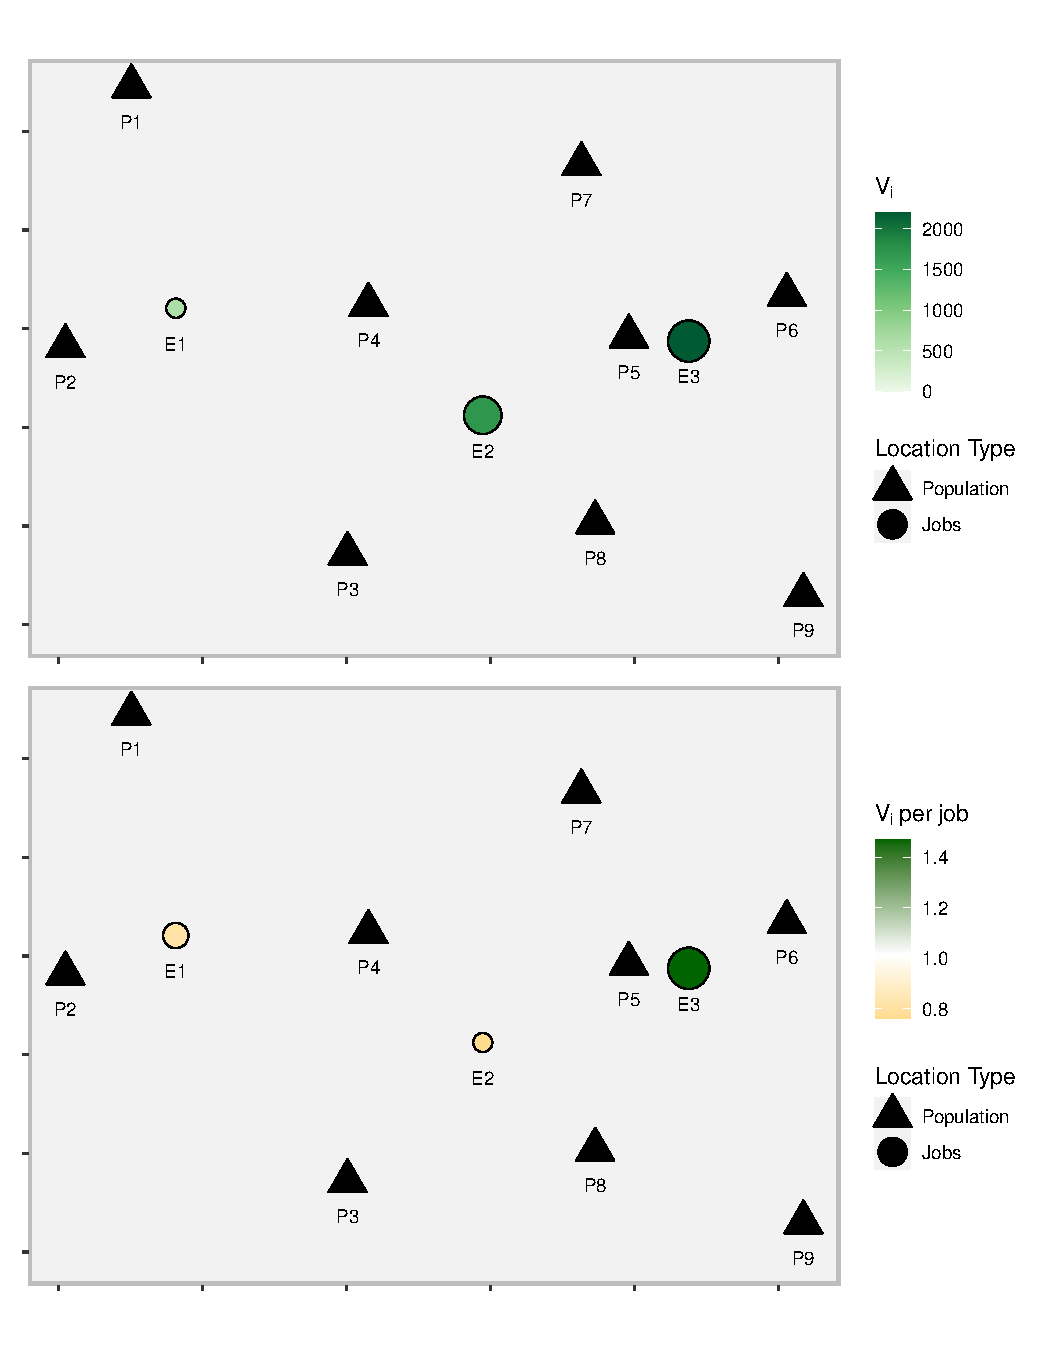
\includegraphics[width=1\linewidth]{Spatial-Availability_files/figure-latex/toy-example-availability-workers-per-job-1} \caption{\label{fig:toy-example-availability-workers-per-job} Spatial availability of workers for each employment center (top) and the spatial availability of workers per job for each employment center (bottom) for the simple synthetic example}\label{fig:toy-example-availability-workers-per-job}
\end{figure}

As shown in Figure \ref{fig:toy-example-availability-workers-per-job},
the top plot demonstrates the spatial availability which measures
accessibility to labor for the three employment centers. As with all
spatial availability calculations, the number of all opportunities (in
this case \emph{workers}) are proportionally allocated to each
employment center so employment center E3, E2 and E1 have access to
2205.19, 1709.52, and 610.29 workers respectively. Again, this totals to
4500 workers in the area. In the bottom plot, these spatial availability
values are normalized per job (i.e.~the `population' of the employment
centers) and we can see that employment center E3 has an above average
worker access of 1.47 workers per job while E2 and E1 have 0.76 and 0.81
workers per job respectively.

\hypertarget{concluding-remarks}{%
\section{Concluding remarks}\label{concluding-remarks}}

In this paper, we introduce a singly-constrained accessibility measure
that we term \emph{spatial availability}. This measure is an alternative
to conventional accessibility calculations that provides more meaningful
estimates than accessibility by ensuring that the estimates match the
observed number of opportunities. This enables the calculation of
per-capita measures and measures relative to regional averages. This
development makes it easier to compare opportunity landscapes across
regions and/or time.

. Spatial availability, however, proportionally allocates opportunities
based on the demand population and travel cost thus constraining the
number of opportunities allocated across the measured region to the
number of opportunities available. This single-sided opportunity
constraint can be said to only consider opportunity competition for any
magnitude of demand population (i.e., when measuring job access per
worker the number of workers (demanding population) does not need to
match the number of jobs (opportunities)).

We demonstrated the use of spatial availability and compared it to
spatial accessibility in an empirical example of workers and jobs in the
GGH. We also discussed two additional use cases to emphasize the
versatility of our new measure. In all examples, we highlight how
intuitive the per demand population access values are and how the can be
interpreted.

Fundamentally, accessibility measure's methodology results in the
overestimation or underestimation of opportunity access as a result of
the competition effect. Accessibility does not include factors to bound
the summation so origins, hypothetically, can have infinite opportunity
access. By including an intuitive single-sided constraint in the new
spatial availability measure, it can be used to calculate access to
non-divisible opportunities. In this paper, we focused on employment,
but any competitive opportunities such as schools, hospitals, and other
essential services with finite capacity at a given time can be studied.
Additionally, opportunities which are non-competitive in the sense that
they have always larger capacities than population can still benefit
from this measure as access will not be over or underestimated as a
result of the competition effect seen in accessibility; non-competitive
opportunities can include large natural parks and beaches. As such,
values measured for opportunities of any type can benefit from an
availability perspective through the reduction in competition effect
(from accessibility) and a meaningful benchmark of demand per population
unit.

\hypertarget{appendix-a}{%
\section{Appendix A}\label{appendix-a}}

\newpage

\begin{figure}

{\centering 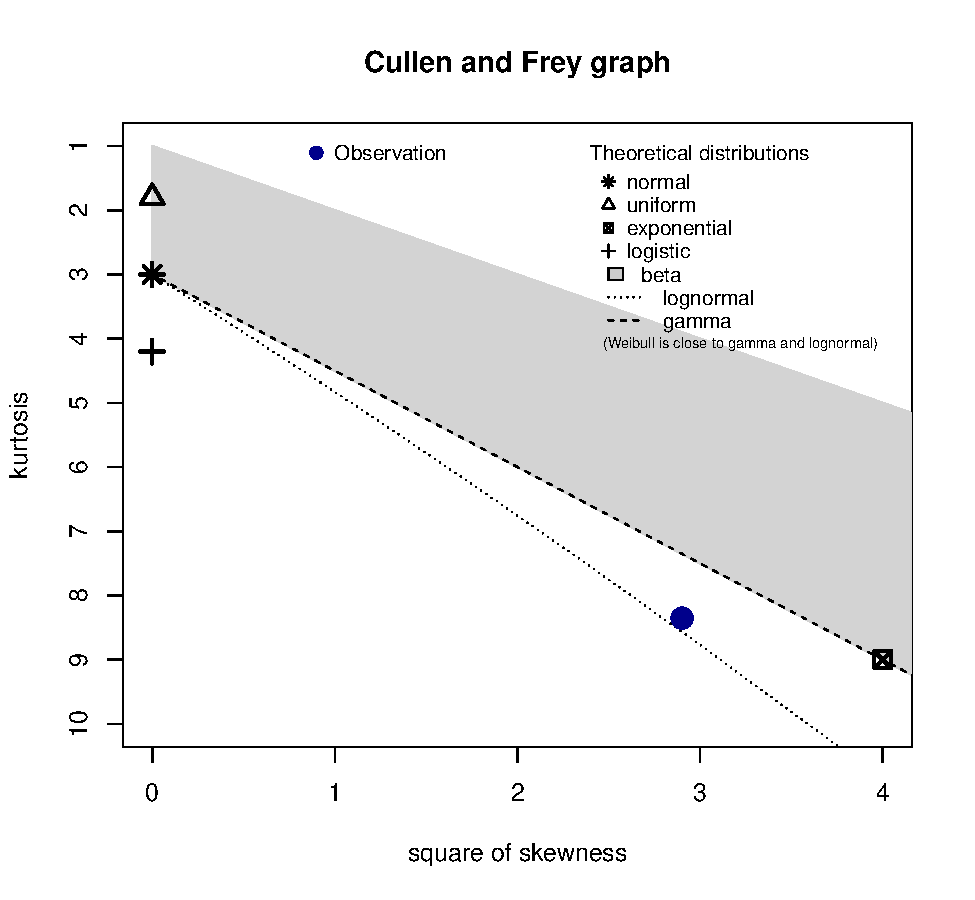
\includegraphics[width=1\linewidth]{Spatial-Availability_files/figure-latex/plot-cullen-frey-1} 

}

\caption{\label{fig:plot-cullen-frey}Cullen and frey graphy for the 2016 TTS calculated travel times.}\label{fig:plot-cullen-frey}
\end{figure}

\hypertarget{references}{%
\section*{References}\label{references}}
\addcontentsline{toc}{section}{References}

\hypertarget{refs}{}
\begin{CSLReferences}{1}{0}
\leavevmode\vadjust pre{\hypertarget{ref-allen2019}{}}%
Allen, J., Farber, S., 2019. A Measure of Competitive Access to
Destinations for Comparing Across Multiple Study Regions. Geographical
Analysis 52, 69--86.
doi:\href{https://doi.org/10.1111/gean.12188}{10.1111/gean.12188}

\leavevmode\vadjust pre{\hypertarget{ref-allen_suburbanization_2021}{}}%
Allen, J., Farber, S., 2021. Suburbanization of {Transport} {Poverty}.
Annals of the American Association of Geographers 111, 18.

\leavevmode\vadjust pre{\hypertarget{ref-Arranz2019measuring}{}}%
Arranz-López, A., Soria-Lara, J.A., Witlox, F., Páez, A., 2019.
Measuring relative non-motorized accessibility to retail activities.
International Journal of Sustainable Transportation 13, 639--651.
doi:\href{https://doi.org/10.1080/15568318.2018.1498563}{10.1080/15568318.2018.1498563}

\leavevmode\vadjust pre{\hypertarget{ref-arribas2021Open}{}}%
Arribas-Bel, D., Green, M., Rowe, F., Singleton, A., 2021. Open data
products-a framework for creating valuable analysis ready data. Journal
of Geographical Systems 23, 497--514.
doi:\href{https://doi.org/10.1007/s10109-021-00363-5}{10.1007/s10109-021-00363-5}

\leavevmode\vadjust pre{\hypertarget{ref-axisa_factors_2012}{}}%
Axisa, J.J., Scott, D.M., Bruce Newbold, K., 2012. Factors influencing
commute distance: A case study of {Toronto}'s commuter shed. Journal of
Transport Geography 24, 123--129.
doi:\href{https://doi.org/10.1016/j.jtrangeo.2011.10.005}{10.1016/j.jtrangeo.2011.10.005}

\leavevmode\vadjust pre{\hypertarget{ref-barboza_balancing_2021}{}}%
Barboza, M.H.C., Carneiro, M.S., Falavigna, C., Luz, G., Orrico, R.,
2021. Balancing time: {Using} a new accessibility measure in {Rio} de
{Janeiro}. Journal of Transport Geography 90, 102924.
doi:\href{https://doi.org/10.1016/j.jtrangeo.2020.102924}{10.1016/j.jtrangeo.2020.102924}

\leavevmode\vadjust pre{\hypertarget{ref-batista_estimation_2019}{}}%
Batista, S.F.A., Leclercq, L., Geroliminis, N., 2019. Estimation of
regional trip length distributions for the calibration of the aggregated
network traffic models. Transportation Research Part B: Methodological
122, 192--217.
doi:\href{https://doi.org/10.1016/j.trb.2019.02.009}{10.1016/j.trb.2019.02.009}

\leavevmode\vadjust pre{\hypertarget{ref-brunsdon2021opening}{}}%
Brunsdon, C., Comber, A., 2021. Opening practice: Supporting
reproducibility and critical spatial data science. Journal of
Geographical Systems 23, 477--496.
doi:\href{https://doi.org/10.1007/s10109-020-00334-2}{10.1007/s10109-020-00334-2}

\leavevmode\vadjust pre{\hypertarget{ref-cervero_transportation_2002}{}}%
Cervero, R., Sandoval, O., Landis, J., 2002. Transportation as a
{Stimulus} of {Welfare}-to-{Work}: {Private} versus {Public} {Mobility}.
Journal of Planning Education and Research 22, 50--63.
doi:\href{https://doi.org/10.1177/0739456X0202200105}{10.1177/0739456X0202200105}

\leavevmode\vadjust pre{\hypertarget{ref-chen_evaluating_2020}{}}%
Chen, B.Y., Cheng, X.-P., Kwan, M.-P., Schwanen, T., 2020. Evaluating
spatial accessibility to healthcare services under travel time
uncertainty: {A} reliability-based floating catchment area approach.
Journal of Transport Geography 87, 102794.
doi:\href{https://doi.org/10.1016/j.jtrangeo.2020.102794}{10.1016/j.jtrangeo.2020.102794}

\leavevmode\vadjust pre{\hypertarget{ref-chen_enhancing_2019}{}}%
Chen, X., 2019. Enhancing the {Two}-{Step} {Floating} {Catchment} {Area}
{Model} for {Community} {Food} {Access} {Mapping}: {Case} of the
{Supplemental} {Nutrition} {Assistance} {Program}. The Professional
Geographer 71, 668--680.
doi:\href{https://doi.org/10.1080/00330124.2019.1578978}{10.1080/00330124.2019.1578978}

\leavevmode\vadjust pre{\hypertarget{ref-chen_spatial_2020}{}}%
Chen, Z., Zhou, X., Yeh, A.G., 2020. Spatial accessibility to
kindergartens using a spectrum combinational approach: {Case} study of
{Shanghai} using cellphone data. Environment and Planning B: Urban
Analytics and City Science 239980832095422.
doi:\href{https://doi.org/10.1177/2399808320954221}{10.1177/2399808320954221}

\leavevmode\vadjust pre{\hypertarget{ref-data_management_group_tts_2018}{}}%
Data Management Group, 2018.
\href{http://dmg.utoronto.ca/transportation-tomorrow-survey/tts-introduction}{{TTS}
- {Transportation} {Tomorrow} {Survey} 2016}.

\leavevmode\vadjust pre{\hypertarget{ref-deboosere2018}{}}%
Deboosere, R., El-Geneidy, A.M., Levinson, D., 2018.
Accessibility-oriented development. Journal of Transport Geography 70,
11--20.
doi:\href{https://doi.org/10.1016/j.jtrangeo.2018.05.015}{10.1016/j.jtrangeo.2018.05.015}

\leavevmode\vadjust pre{\hypertarget{ref-delamater2013spatial}{}}%
Delamater, P.L., 2013. Spatial accessibility in suboptimally configured
health care systems: A modified two-step floating catchment area
(M2SFCA) metric. Health \& Place 24, 30--43.
doi:\href{https://doi.org/10.1016/j.healthplace.2013.07.012}{10.1016/j.healthplace.2013.07.012}

\leavevmode\vadjust pre{\hypertarget{ref-fitdistrplus_2015}{}}%
Delignette-Muller, M.L., Dutang, C., 2015.
\href{https://www.jstatsoft.org/article/view/v064i04}{{fitdistrplus}: An
{R} package for fitting distributions}. Journal of Statistical Software
64, 1--34.

\leavevmode\vadjust pre{\hypertarget{ref-elgeneidy_cost_2016}{}}%
El-Geneidy, A., Levinson, D., Diab, E., Boisjoly, G., Verbich, D.,
Loong, C., 2016. The cost of equity: {Assessing} transit accessibility
and social disparity using total travel cost. Transportation Research
Part A: Policy and Practice 91, 302--316.
doi:\href{https://doi.org/10.1016/j.tra.2016.07.003}{10.1016/j.tra.2016.07.003}

\leavevmode\vadjust pre{\hypertarget{ref-geurs2004}{}}%
Geurs, K.T., van Wee, B., 2004. Accessibility evaluation of land-use and
transport strategies: review and research directions. Journal of
Transport Geography 12, 127--140.
doi:\href{https://doi.org/10.1016/j.jtrangeo.2003.10.005}{10.1016/j.jtrangeo.2003.10.005}

\leavevmode\vadjust pre{\hypertarget{ref-handy2020}{}}%
Handy, S., 2020. Is accessibility an idea whose time has finally come?
Transportation Research Part D: Transport and Environment 83, 102319.
doi:\href{https://doi.org/10.1016/j.trd.2020.102319}{10.1016/j.trd.2020.102319}

\leavevmode\vadjust pre{\hypertarget{ref-handy_measuring_1997}{}}%
Handy, S.L., Niemeier, D.A., 1997. Measuring {Accessibility}: {An}
{Exploration} of {Issues} and {Alternatives}. Environment and Planning
A: Economy and Space 29, 1175--1194.
doi:\href{https://doi.org/10.1068/a291175}{10.1068/a291175}

\leavevmode\vadjust pre{\hypertarget{ref-hansen1959}{}}%
Hansen, W.G., 1959. How Accessibility Shapes Land Use. Journal of the
American Institute of Planners 25, 73--76.
doi:\href{https://doi.org/10.1080/01944365908978307}{10.1080/01944365908978307}

\leavevmode\vadjust pre{\hypertarget{ref-higgins2019}{}}%
Higgins, C.D., 2019. Accessibility toolbox for r and ArcGIS. Transport
Findings. doi:\href{https://doi.org/10.32866/8416}{10.32866/8416}

\leavevmode\vadjust pre{\hypertarget{ref-higgins2021changes}{}}%
Higgins, C.D., Páez, A., Ki, G., Wang, J., 2021. Changes in
accessibility to emergency and community food services during COVID-19
and implications for low income populations in hamilton, ontario. Social
Science \& Medicine 114442.
doi:\href{https://doi.org/10.1016/j.socscimed.2021.114442}{10.1016/j.socscimed.2021.114442}

\leavevmode\vadjust pre{\hypertarget{ref-horbachov_theoretical_2018}{}}%
Horbachov, P., Svichynskyi, S., 2018.
\href{https://www.jstor.org/stable/26622420}{Theoretical substantiation
of trip length distribution for home-based work trips in urban transit
systems}. Journal of Transport and Land Use 11, 593--632.

\leavevmode\vadjust pre{\hypertarget{ref-joseph1984}{}}%
Joseph, A.E., Bantock, P.R., 1984. Rural Accessibility of General
Practitioners: the Case of Bruce and Grey Counties, ONTARIO,
1901{\textendash}1981. The Canadian Geographer/Le Géographe canadien 28,
226--239.
doi:\href{https://doi.org/10.1111/j.1541-0064.1984.tb00788.x}{10.1111/j.1541-0064.1984.tb00788.x}

\leavevmode\vadjust pre{\hypertarget{ref-kwan_spacetime_1998}{}}%
Kwan, M.-P., 1998. Space-{Time} and {Integral} {Measures} of
{Individual} {Accessibility}: {A} {Comparative} {Analysis} {Using} a
{Point}-based {Framework}. Geographical Analysis 30, 191--216.
doi:\href{https://doi.org/10.1111/j.1538-4632.1998.tb00396.x}{10.1111/j.1538-4632.1998.tb00396.x}

\leavevmode\vadjust pre{\hypertarget{ref-levinson_accessibility_1998}{}}%
Levinson, D.M., 1998. Accessibility and the journey to work. Journal of
Transport Geography 6, 11--21.
doi:\href{https://doi.org/10.1016/S0966-6923(97)00036-7}{10.1016/S0966-6923(97)00036-7}

\leavevmode\vadjust pre{\hypertarget{ref-li_approach_2020}{}}%
Li, A., Huang, Y., Axhausen, K.W., 2020. An approach to imputing
destination activities for inclusion in measures of bicycle
accessibility. Journal of Transport Geography 82, 102566.
doi:\href{https://doi.org/10.1016/j.jtrangeo.2019.102566}{10.1016/j.jtrangeo.2019.102566}

\leavevmode\vadjust pre{\hypertarget{ref-luo2003}{}}%
Luo, W., Wang, F., 2003. Measures of Spatial Accessibility to Health
Care in a GIS Environment: Synthesis and a Case Study in the Chicago
Region. Environment and Planning B: Planning and Design 30, 865--884.
doi:\href{https://doi.org/10.1068/b29120}{10.1068/b29120}

\leavevmode\vadjust pre{\hypertarget{ref-miller2018}{}}%
Miller, E.J., 2018. Accessibility: measurement and application in
transportation planning. Transport Reviews 38, 551--555.
doi:\href{https://doi.org/10.1080/01441647.2018.1492778}{10.1080/01441647.2018.1492778}

\leavevmode\vadjust pre{\hypertarget{ref-paez2004network}{}}%
Paez, A., 2004. Network accessibility and the spatial distribution of
economic activity in eastern asia. Urban Studies 41, 2211--2230.

\leavevmode\vadjust pre{\hypertarget{ref-paez2019}{}}%
Paez, A., Higgins, C.D., Vivona, S.F., 2019. Demand and level of service
inflation in Floating Catchment Area (FCA) methods. PLOS ONE 14,
e0218773.
doi:\href{https://doi.org/10.1371/journal.pone.0218773}{10.1371/journal.pone.0218773}

\leavevmode\vadjust pre{\hypertarget{ref-paez2012measuring}{}}%
Paez, A., Scott, D.M., Morency, C., 2012. Measuring accessibility:
Positive and normative implementations of various accessibility
indicators. Journal of Transport Geography 25, 141--153.
doi:\href{https://doi.org/10.1016/j.jtrangeo.2012.03.016}{10.1016/j.jtrangeo.2012.03.016}

\leavevmode\vadjust pre{\hypertarget{ref-paez2021open}{}}%
Páez, A., 2021. Open spatial sciences: An introduction. Journal of
Geographical Systems 23, 467--476.
doi:\href{https://doi.org/10.1007/s10109-021-00364-4}{10.1007/s10109-021-00364-4}

\leavevmode\vadjust pre{\hypertarget{ref-paez_jobs_2013}{}}%
Páez, A., Farber, S., Mercado, R., Roorda, M., Morency, C., 2013. Jobs
and the {Single} {Parent}: {An} {Analysis} of {Accessibility} to
{Employment} in {Toronto}. Urban Geography 34, 815--842.
doi:\href{https://doi.org/10.1080/02723638.2013.778600}{10.1080/02723638.2013.778600}

\leavevmode\vadjust pre{\hypertarget{ref-pereira_distributional_2019}{}}%
Pereira, R.H.M., Banister, D., Schwanen, T., Wessel, N., 2019.
Distributional effects of transport policies on inequalities in access
to opportunities in {Rio} de {Janeiro}. Journal of Transport and Land
Use 12.
doi:\href{https://doi.org/10.5198/jtlu.2019.1523}{10.5198/jtlu.2019.1523}

\leavevmode\vadjust pre{\hypertarget{ref-proffitt2017}{}}%
Proffitt, D.G., Bartholomew, K., Ewing, R., Miller, H.J., 2017.
Accessibility planning in American metropolitan areas: Are we there yet?
Urban Studies 56, 167--192.
doi:\href{https://doi.org/10.1177/0042098017710122}{10.1177/0042098017710122}

\leavevmode\vadjust pre{\hypertarget{ref-qi_decadelong_2018}{}}%
Qi, Y., Fan, Y., Sun, T., Hu, L.(Ivy)., 2018. Decade-long changes in
spatial mismatch in {Beijing}, {China}: {Are} disadvantaged populations
better or worse off? Environment and Planning A: Economy and Space 50,
848--868.
doi:\href{https://doi.org/10.1177/0308518X18755747}{10.1177/0308518X18755747}

\leavevmode\vadjust pre{\hypertarget{ref-r5r_2021}{}}%
Rafael H. M. Pereira, Marcus Saraiva, Daniel Herszenhut, Carlos Kaue
Vieira Braga, Matthew Wigginton Conway, 2021. r5r: Rapid realistic
routing on multimodal transport networks with R5 in r. Findings.
doi:\href{https://doi.org/10.32866/001c.21262}{10.32866/001c.21262}

\leavevmode\vadjust pre{\hypertarget{ref-reggiani_accessibility_2011}{}}%
Reggiani, A., Bucci, P., Russo, G., 2011. Accessibility and {Impedance}
{Forms}: {Empirical} {Applications} to the {German} {Commuting}
{Network}. International Regional Science Review 34, 230--252.
doi:\href{https://doi.org/10.1177/0160017610387296}{10.1177/0160017610387296}

\leavevmode\vadjust pre{\hypertarget{ref-rosik_forecast_2021}{}}%
Rosik, P., Goliszek, S., Komornicki, T., Duma, P., 2021. Forecast of the
{Impact} of {Electric} {Car} {Battery} {Performance} and
{Infrastructural} and {Demographic} {Changes} on {Cumulative}
{Accessibility} for the {Five} {Most} {Populous} {Cities} in {Poland}.
Energies 14, 8350.
doi:\href{https://doi.org/10.3390/en14248350}{10.3390/en14248350}

\leavevmode\vadjust pre{\hypertarget{ref-santanapalacios2022}{}}%
Santana Palacios, M., El-geneidy, A., 2022. Cumulative versus
Gravity-based Accessibility Measures: Which One to Use? Findings.
doi:\href{https://doi.org/10.32866/001c.32444}{10.32866/001c.32444}

\leavevmode\vadjust pre{\hypertarget{ref-shen1998}{}}%
Shen, Q., 1998. Location characteristics of inner-city neighborhoods and
employment accessibility of low-wage workers. Environment and Planning
B: Planning and Design 25, 345--365.
doi:\href{https://doi.org/10.1068/b250345}{10.1068/b250345}

\leavevmode\vadjust pre{\hypertarget{ref-shi_literature_2020}{}}%
Shi, Y., Blainey, S., Sun, C., Jing, P., 2020. A literature review on
accessibility using bibliometric analysis techniques. Journal of
Transport Geography 87, 102810.
doi:\href{https://doi.org/10.1016/j.jtrangeo.2020.102810}{10.1016/j.jtrangeo.2020.102810}

\leavevmode\vadjust pre{\hypertarget{ref-vale_influence_2017}{}}%
Vale, D.S., Pereira, M., 2017. The influence of the impedance function
on gravity-based pedestrian accessibility measures: {A} comparative
analysis. Environment and Planning B: Urban Analytics and City Science
44, 740--763.
doi:\href{https://doi.org/10.1177/0265813516641685}{10.1177/0265813516641685}

\leavevmode\vadjust pre{\hypertarget{ref-wan2012three}{}}%
Wan, N., Zou, B., Sternberg, T., 2012. A three-step floating catchment
area method for analyzing spatial access to health services.
International Journal of Geographical Information Science 26,
1073--1089.
doi:\href{https://doi.org/10.1080/13658816.2011.624987}{10.1080/13658816.2011.624987}

\leavevmode\vadjust pre{\hypertarget{ref-wang_access_2021}{}}%
Wang, S., Wang, M., Liu, Y., 2021. Access to urban parks: {Comparing}
spatial accessibility measures using three {GIS}-based approaches.
Computers, Environment and Urban Systems 90, 101713.
doi:\href{https://doi.org/10.1016/j.compenvurbsys.2021.101713}{10.1016/j.compenvurbsys.2021.101713}

\leavevmode\vadjust pre{\hypertarget{ref-wilson1971}{}}%
Wilson, A.G., 1971. A Family of Spatial Interaction Models, and
Associated Developments. Environment and Planning A: Economy and Space
3, 1--32. doi:\href{https://doi.org/10.1068/a030001}{10.1068/a030001}

\leavevmode\vadjust pre{\hypertarget{ref-yan2021}{}}%
Yan, X., 2021. Toward Accessibility-Based Planning. Journal of the
American Planning Association 87, 409--423.
doi:\href{https://doi.org/10.1080/01944363.2020.1850321}{10.1080/01944363.2020.1850321}

\leavevmode\vadjust pre{\hypertarget{ref-yang_comparing_2006}{}}%
Yang, D.-H., Goerge, R., Mullner, R., 2006. Comparing {GIS}-{Based}
{Methods} of {Measuring} {Spatial} {Accessibility} to {Health}
{Services}. Journal of Medical Systems 30, 23--32.
doi:\href{https://doi.org/10.1007/s10916-006-7400-5}{10.1007/s10916-006-7400-5}

\leavevmode\vadjust pre{\hypertarget{ref-ye_spatial_2018}{}}%
Ye, C., Zhu, Y., Yang, J., Fu, Q., 2018. Spatial equity in accessing
secondary education: {Evidence} from a gravity-based model: {Spatial}
equity in accessing secondary education. The Canadian Geographer / Le
Géographe canadien 62, 452--469.
doi:\href{https://doi.org/10.1111/cag.12482}{10.1111/cag.12482}

\end{CSLReferences}


\end{document}
